\documentclass[a4paper,11pt]{book}

%%%%%%%%%%%%%%%%%%%%%%%%%%%%%%%%%
% Paquetes
%%%%%%%%%%%%%%%%%%%%%%%%%%%%%%%%%
\usepackage[utf8]{inputenc}
\usepackage[spanish]{babel}
\usepackage{csquotes}
\usepackage[inline]{enumitem}
\usepackage{graphicx}
\usepackage[official]{eurosym}
\usepackage{listings}
\usepackage{multirow}
% \usepackage{float}

\decimalpoint
\usepackage{dcolumn}
\newcolumntype{.}{D{.}{\esperiod}{-1}}
\makeatletter
\addto\shorthandsspanish{\let\esperiod\es@period@code}
\makeatother

\RequirePackage{verbatim}
\usepackage{fancyhdr}
\usepackage{afterpage}
\usepackage{longtable}
\usepackage[pdfborder={0 0 0}]{hyperref} %referencia
\usepackage{url}
\usepackage{colortbl}
\usepackage[stable]{footmisc}
\usepackage{pdfpages}

% ********************************************************************
% Re-usable information
% ********************************************************************

\newcommand{\myTitle}{Desarrollo de un instrumento musical digital\xspace}
\newcommand{\myDegree}{Grado en Ingeniería Informática\xspace}
\newcommand{\myName}{Jesús Jiménez Sánchez (alumno)\xspace}
\newcommand{\myProf}{Alberto Guillén Perales (tutor1)\xspace}
%\newcommand{\mySupervisor}{Put name here\xspace}
\newcommand{\myFaculty}{Escuela Técnica Superior de Ingenierías Informática y de Telecomunicación\xspace}
\newcommand{\myFacultyShort}{E.T.S. de Ingenierías Informática y de Telecomunicación\xspace}
\newcommand{\myDepartment}{Departamento de ...\xspace}
\newcommand{\myUni}{\protect{Universidad de Granada}\xspace}
\newcommand{\myLocation}{Granada\xspace}
\newcommand{\myTime}{\today\xspace}
\newcommand{\myVersion}{Version 0.1\xspace}


%%%%%%%%%%%%%%%%%%%%%%%%%%%
% Preparar pdf
%%%%%%%%%%%%%%%%%%%%%%%%%%%

\hypersetup{
    pdfauthor = {\myName (jesusjimsa@correo.ugr.es)},
    pdftitle = {\myTitle},
    pdfsubject = {},
    pdfkeywords = {palabraclave1, palabraclave2, palabraclave3, ...},
    pdfcreator = {LaTeX con el paquete ....},
    pdfproducer = {pdflatex}
}


% Comandos útiles
\pagestyle{fancy}
\fancyhf{}
\fancyhead[LO]{\leftmark}
\fancyhead[RE]{\rightmark}
\fancyhead[RO,LE]{\textbf{\thepage}}
\renewcommand{\chaptermark}[1]{\markboth{\textbf{#1}}{}}
\renewcommand{\sectionmark}[1]{\markright{\textbf{\thesection. #1}}}

\setlength{\headheight}{1.5\headheight}

\newcommand{\HRule}{\rule{\linewidth}{0.5mm}}
% Definimos los tipos teorema, ejemplo y definición podremos usar estos tipos
% simplemente poniendo \begin{teorema} \end{teorema} ...
\newtheorem{teorema}{Teorema}[chapter]
\newtheorem{ejemplo}{Ejemplo}[chapter]
\newtheorem{definicion}{Definición}[chapter]

\definecolor{gray97}{gray}{.97}
\definecolor{gray75}{gray}{.75}
\definecolor{gray45}{gray}{.45}
\definecolor{gray30}{gray}{.94}

\lstset{
    frame=Ltb,
    framerule=0.5pt,
    aboveskip=0.5cm,
    framextopmargin=3pt,
    framexbottommargin=3pt,
    framexleftmargin=0.1cm,
    framesep=0pt,
    rulesep=.4pt,
    backgroundcolor=\color{gray97},
    rulesepcolor=\color{black},
    %
    stringstyle=\ttfamily,
    showstringspaces = false,
    basicstyle=\scriptsize\ttfamily,
    commentstyle=\color{gray45},
    keywordstyle=\bfseries,
    %
    numbers=left,
    numbersep=6pt,
    numberstyle=\tiny,
    numberfirstline = false,
    breaklines=true,
}

% minimizar fragmentado de listados
\lstnewenvironment{listing}[1][]
   {\lstset{#1}\pagebreak[0]}{\pagebreak[0]}

\lstdefinestyle{CodigoC}
{
    basicstyle=\scriptsize,
    frame=single,
    language=C,
    numbers=left
}

\lstdefinestyle{CodigoC++}
{
    basicstyle=\small,
    frame=single,
    backgroundcolor=\color{gray30},
    language=C++,
    numbers=left
}

\lstdefinestyle{Consola}
{
    basicstyle=\scriptsize\bf\ttfamily,
    backgroundcolor=\color{gray30},
    frame=single,
    numbers=none
}


\newcommand{\bigrule}{\titlerule[0.5mm]}

%Para conseguir que en las páginas en blanco no ponga cabecerass
\makeatletter
\def\clearpage{%
    \ifvmode
        \ifnum \@dbltopnum =\m@ne
        \ifdim \pagetotal <\topskip
            \hbox{}
        \fi
        \fi
    \fi
    \newpage
    \thispagestyle{empty}
    \write\m@ne{}
    \vbox{}
    \penalty -\@Mi
}
\makeatother

%%%%%%%%%%%%%%%%%%%%%%%%%%%%%%%%%%
% Imagenes
%%%%%%%%%%%%%%%%%%%%%%%%%%%%%%%%%%
\graphicspath{ {./imagenes/} }


\title{ \myTitle }
\author{ \myName }

\begin{document}

\begin{titlepage}
 
 
\newlength{\centeroffset}
\setlength{\centeroffset}{-0.5\oddsidemargin}
\addtolength{\centeroffset}{0.5\evensidemargin}
\thispagestyle{empty}

\noindent\hspace*{\centeroffset}\begin{minipage}{\textwidth}

\centering

\includegraphics[width=0.9\textwidth]{logo_ugr.jpg}\\[1.4cm]

\textsc{ \Large TRABAJO FIN DE GRADO\\[0.2cm]}
\textsc{ INGENIERÍA EN INGENIERÍA INFORMÁTICA}\\[1cm]
% Upper part of the page
% 
% Title
{\Huge\bfseries Desarrollo de un instrumento musical digital\\
}
\noindent\rule[-1ex]{\textwidth}{3pt}\\[3.5ex]
{\large\bfseries Subtitulo del Proyecto}
\end{minipage}

\vspace{2.5cm}
\noindent\hspace*{\centeroffset}\begin{minipage}{\textwidth}
\centering

\textbf{Autor}\\ { Jesús Jiménez Sánchez (alumno) }\\[2.5ex]
\textbf{Directores}\\
{ Alberto Guillén Perales \\[2cm] }

\includegraphics[width=0.3\textwidth]{etsiit_logo.png}\\[0.1cm]
\textsc{Escuela Técnica Superior de Ingenierías Informática y de Telecomunicación}\\
\textsc{---}\\
Granada, mes de 201
\end{minipage}

\end{titlepage}



%%%%%%%%%%%%%%%%%%%%%%%%%%%%%%%%%%%%%%%%%%%%%%%%%%%%%%%%%%%%%%%%%%%%%%%%%%%%%%%%%
% Prefacio
%%%%%%%%%%%%%%%%%%%%%%%%%%%%%%%%%%%%%%%%%%%%%%%%%%%%%%%%%%%%%%%%%%%%%%%%%%%%%%%%%

\chapter*{}   %%%%%%%%%%%%%%%%%%%%%%

\cleardoublepage
\thispagestyle{empty}

\begin{center}
    {\large\bfseries Desarrollo de un instrumento musical digital}\\
\end{center}

\begin{center}
    Jesús Jiménez Sánchez\\
\end{center}

%\vspace{0.7cm}
\noindent{\textbf{Palabras clave}: batería, sonido, Raspberry, Arduino, ......}\\

\vspace{0.7cm}
\noindent{\textbf{Resumen}}\\

Poner aquí el resumen.

\cleardoublepage

\thispagestyle{empty}

\begin{center}
       {\large\bfseries Development of a digital musical instrument}\\
\end{center}

\begin{center}
    Jesús Jiménez Sánchez\\
\end{center}

\noindent{\textbf{Keywords}: batería, sonido, Raspberry, Arduino, ....}\\

\vspace{0.7cm}
\noindent{\textbf{Abstract}}\\

Write here the abstract in English.

\chapter*{}   %%%%%%%%%%%%%%%%%%%%%%

\thispagestyle{empty}

\noindent\rule[-1ex]{\textwidth}{2pt}\\[4.5ex]

Yo, \textbf{Jesús Jiménez Sánchez}, alumno de la titulación \textbf{Grado en Ingeniería Informática} de la
\textbf{Escuela Técnica Superior de Ingenierías Informática y de Telecomunicación de la Universidad de Granada}, con DNI
11111111A, autorizo la ubicación de la siguiente copia de mi Trabajo Fin de Grado en la biblioteca del centro para que
pueda ser consultada por las personas que lo deseen.

\vspace{6cm}

\noindent Fdo: Jesús Jiménez Sánchez

\vspace{2cm}

\begin{flushright}
    Granada a X de mes de 2020.
\end{flushright}

\chapter*{}   %%%%%%%%%%%%%%%%%%%%%%
\thispagestyle{empty}

\noindent\rule[-1ex]{\textwidth}{2pt}\\[4.5ex]

D. \textbf{Alberto Guillén Perales}, Profesor del Área de XXXX del Departamento YYYY de la Universidad de
Granada.

\vspace{0.5cm}

\textbf{Informan:}

\vspace{0.5cm}

Que el presente trabajo, titulado \textit{\textbf{Desarrollo de un instrumento musical digital}},
ha sido realizado bajo su supervisión por \textbf{Jesús Jiménez Sánchez}, y autorizamos la defensa de
dicho trabajo ante el tribunal
que corresponda.

\vspace{0.5cm}

Y para que conste, expiden y firman el presente informe en Granada a X de mes de 201 .

\vspace{1cm}

\textbf{Los directores:}

\vspace{5cm}

\noindent \textbf{Alberto Guillén Perales}

\chapter*{Agradecimientos}  %%%%%%%%%%%%%%%%%%%%%%
\thispagestyle{empty}

    \vspace{1cm}


Poner aquí agradecimientos...


\newpage
\tableofcontents
\newpage
\listoffigures
\newpage

%%%%%%%%%%%%%%%%%%%%%%%%%%%%%%%%%%%%%%%%%%%%%%%%%%%%%%%%%%%%%%%%%%%%%%%%%%%%%%%%%
% Objetivos
%%%%%%%%%%%%%%%%%%%%%%%%%%%%%%%%%%%%%%%%%%%%%%%%%%%%%%%%%%%%%%%%%%%%%%%%%%%%%%%%%

\chapter{Objetivos} % (fold)
\label{cha:Objetivos}

    Objetivo General:

    Objetivos específicos:
    \begin{itemize}
        \item OB-E1: Planificación
        \item OB-E2:
    \end{itemize}

% chapter Objetivos (end)


%%%%%%%%%%%%%%%%%%%%%%%%%%%%%%%%%%%%%%%%%%%%%%%%%%%%%%%%%%%%%%%%%%%%%%%%%%%%%%%%%
% Introducción
%%%%%%%%%%%%%%%%%%%%%%%%%%%%%%%%%%%%%%%%%%%%%%%%%%%%%%%%%%%%%%%%%%%%%%%%%%%%%%%%%

\chapter{Introducción} % (fold)
\label{cha:Introduccion}

    \section{Historia de los instrumentos digitales} % (fold)
    \label{sec:HistoriaDeLosInstrumentosDigitales}

        Los primeros intentos de guardar y reproducir el sonido fueron analógicos. Estos métodos captan las ondas y las
        almacenan en diferentes medios para su posterior reproducción, como en un disco de vinilo o un casete.

        Con la aparición de la informática y los ordenadores se empiezan a almacenar estos sonidos en un formato
        digital, capaz de ser interpretado por ordenadores. En este caso, los sonidos se guardan en forma de bytes en
        diferentes formatos de archivo, como MP3, AAC, OGG...

        Los primeros intentos de instrumento musical no analógico se pueden encontrar en los sintetizadores. Estos
        intrumentos utilizan la electricidad para producir las ondas del sonidos pasándola por una serie de módulos.
        Hasta la década de 1980, cada fabricante utilizaba su propio estándar para la sincronización de los sonidos de
        los sintetizadores. En 1981, la empresa Oberheim Electronics comenzó a contactar con otros fabricantes para
        desarrollar un estándar, de ese modo apareció MIDI. Este estándar describe el protocolo de comunicación, la
        interfaz digital y las conexiones electrónicas que deben llevar los diferentes tipos de dispositivos
        electrónicos para reproducir, editar y grabar música \cite{midi_wikipedia}.

        En cuanto a instrumentos musicales electrónicos podemos encontrar desde un teclado o una guitarra a una batería.

        En el área de instrumentos digitales nos encontramos con los instrumentos VST (Virtual Studio Technology). Estos
        instrumentos toman muestras de sonidos de diferentes instrumentos y, mediante un teclado y un ordenador,
        programar estos sonidos y componer y grabar cualquier tipo de canción \cite{historia_instrumentos_digitales}.

        \newpage

        \begin{figure}[ht]
            \centering
            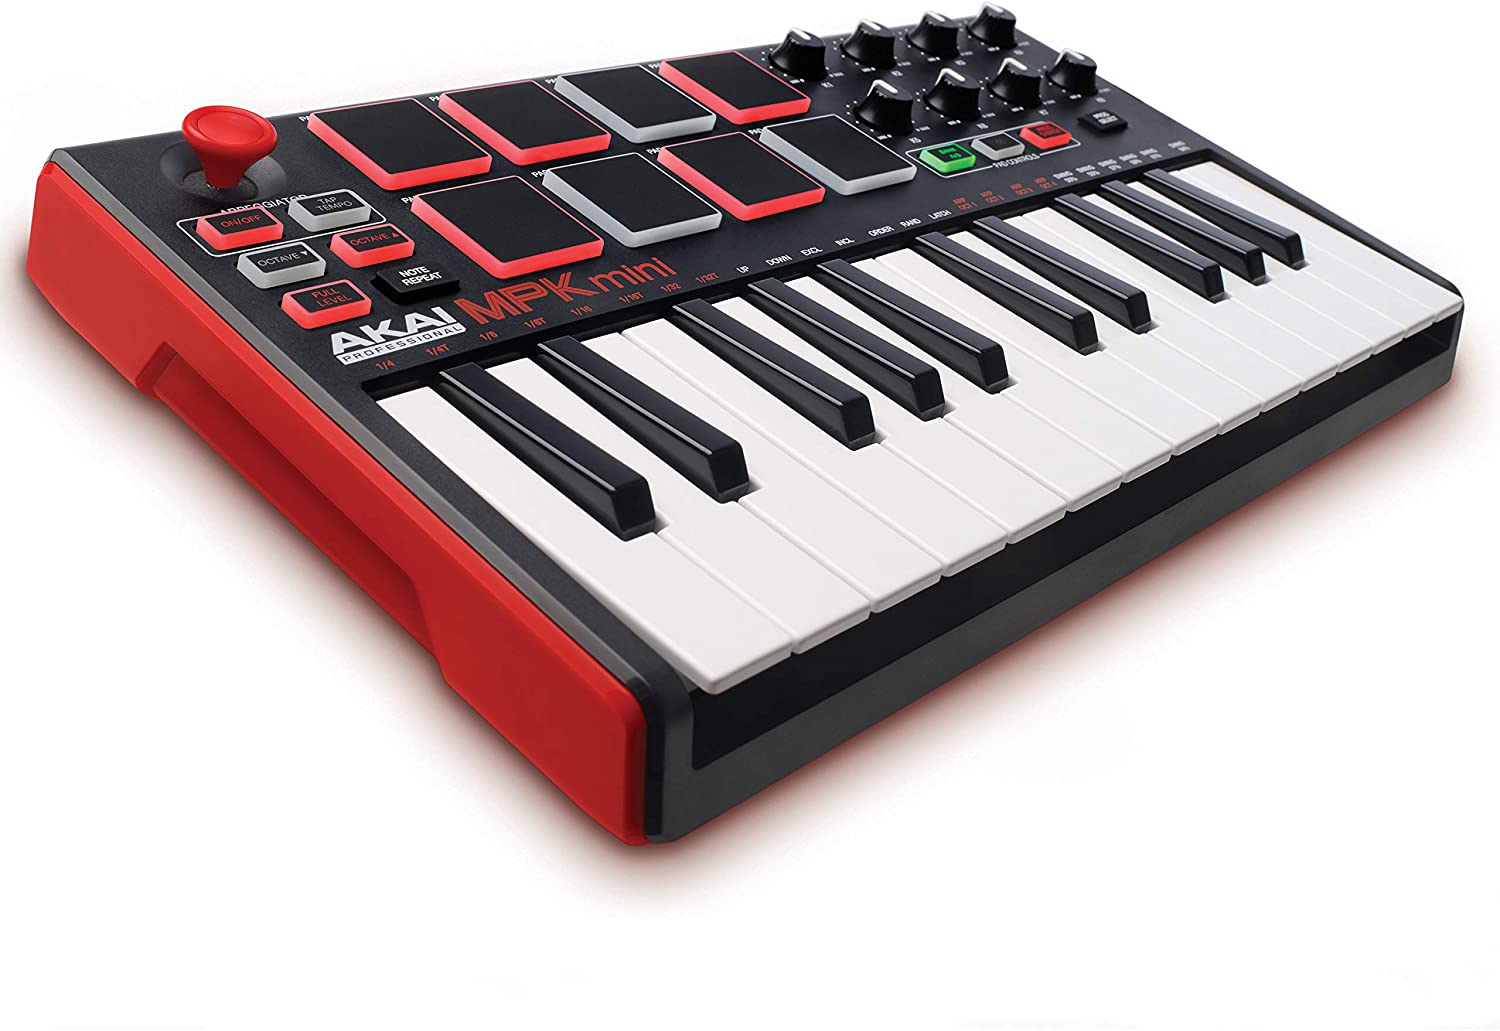
\includegraphics[width=\textwidth/2]{ejemplo_sampler}
            \caption{Ejemplo de sampler digital de la marca AKAI Pro \cite{akai_pro_imagen}\label{fig:EjemploSampler}}
        \end{figure}

    % section Historia de los instrumentos digitales (end)

    \section{Partes de una batería} % (fold)
    \label{sec:PartesDeUnaBateria}

        Las partes de una batería son las siguientes:

        \begin{itemize}
            \item \textbf{Caja}: Su función principal suele ser la de marcar los compases.
            \item \textbf{Toms}: Son los tambores más numerosos en una batería.
            \item \textbf{Bombo}: Se toca con un pedal y produce el sonido más grave de la batería. Se utiliza para
            llevar la base del ritmo.
            \item \textbf{Platillo crash}: Se utiliza para dar énfasis y suele ir acompañado del bombo.
            \item \textbf{Platillo hi-hat}: Consta de dos platillos que se pueden abrir o cerrar con un pedal y se
            utiliza para llevar el ritmo de la canción.
            \item \textbf{Platillo ride}: Puede usarse para llevar el ritmo en lugar de con el hi-hat.
        \end{itemize}

        \newpage

        \begin{figure}[ht]
            \centering
            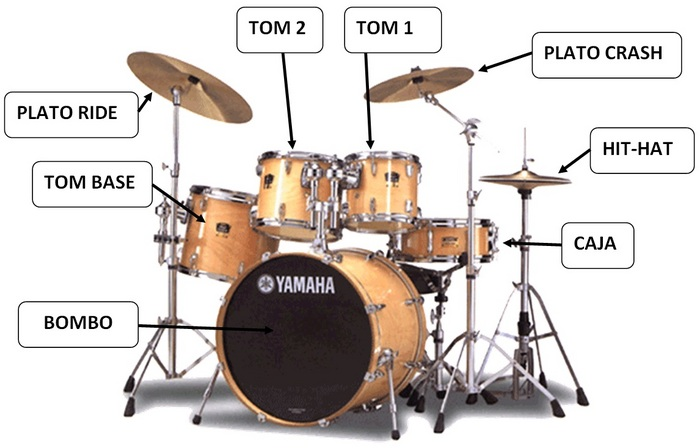
\includegraphics[width=10cm]{partes_bateria}
            \caption{Partes de una batería \cite{partes_bateria_fuente}\label{fig:PartesBateria}}
        \end{figure}

    % section Partes de una batería (end)

    \section{Etapas} % (fold)
    \label{sec:Etapas}

        \begin{itemize}
            \item \textbf{1ª etapa:} Estudio del problema.

            \item \textbf{2ª etapa:} Búsqueda de bibliotecas de reproducción de sonido.

            \item \textbf{3ª etapa:} Implementación del software.

            \item \textbf{4 a etapa:} Construcción de la batería.

            \item \textbf{5ª etapa:} Documentación.
        \end{itemize}

    % section Etapas (end)

    \section{Planificación} % (fold)
    \label{sec:Planificacion}

        \subsection{A priori optimista} % (fold)
        \label{sub:APrioriOptimista}

            \begin{figure}[ht]
                \centering
                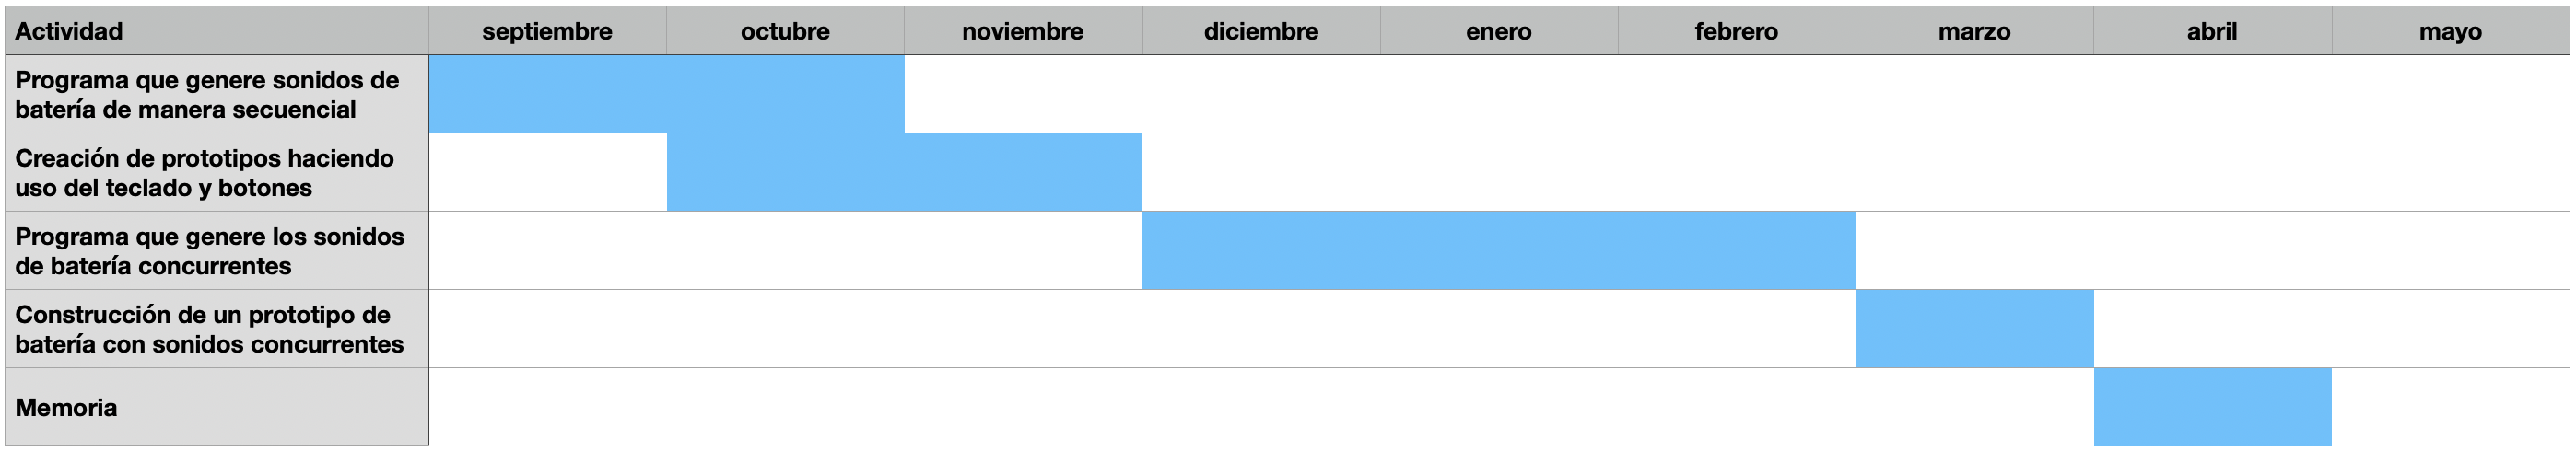
\includegraphics[width=\textwidth]{planificacion_gantt}
                \caption{Diagrama de Gantt de la planificación por etapas\label{fig:PlanificacionGantt}}
            \end{figure}

        % subsection A priori optimista (end)

        % \subsection{A posteriori (en caso de haber diferencias)} % (fold)
        % \label{sub:APosterioriEnCasoDeHaberDiferencias)}

        % subsection A posteriori (en caso de haber diferencias) (end)

    % section Planificación (end)

% chapter Introducción (end)

\newpage

%%%%%%%%%%%%%%%%%%%%%%%%%%%%%%%%%%%%%%%%%%%%%%%%%%%%%%%%%%%%%%%%%%%%%%%%%%%%%%%%%
% Introducción
%%%%%%%%%%%%%%%%%%%%%%%%%%%%%%%%%%%%%%%%%%%%%%%%%%%%%%%%%%%%%%%%%%%%%%%%%%%%%%%%%

\chapter{Estado del arte} % (fold)
\label{sec:EstadoDelArte}

    Este capítulo se encarga de introducir las dos placas utilizadas en el proyecto, explicar las opciones actuales en
    el mercado en cuanto a baterías electricas y realizar la propuesta de batería que se llevará a cabo.

    \section{Raspberry Pi} % (fold)
    \label{sec:RaspberryPi}

        \subsection{¿Qué es Raspberry Pi?} % (fold)
        \label{sub:QueEsRaspberryPi}

            ``Es un ordenador del tamaño de una tarjeta de crédito. Consta de una placa base sobre la que se monta un
            procesador, un chip gráfico y memoria RAM. Fue lanzado en 2006 por la Fundación Raspberry Pi con el objeto
            de estimular la enseñanza de informática en las escuelas de todo el mundo.''

            \begin{flushright}
                (El Confidencial, 22 de Noviembre de 2013. \cite{confidencial_raspberry})
            \end{flushright}

            \begin{figure}[ht]
                \centering
                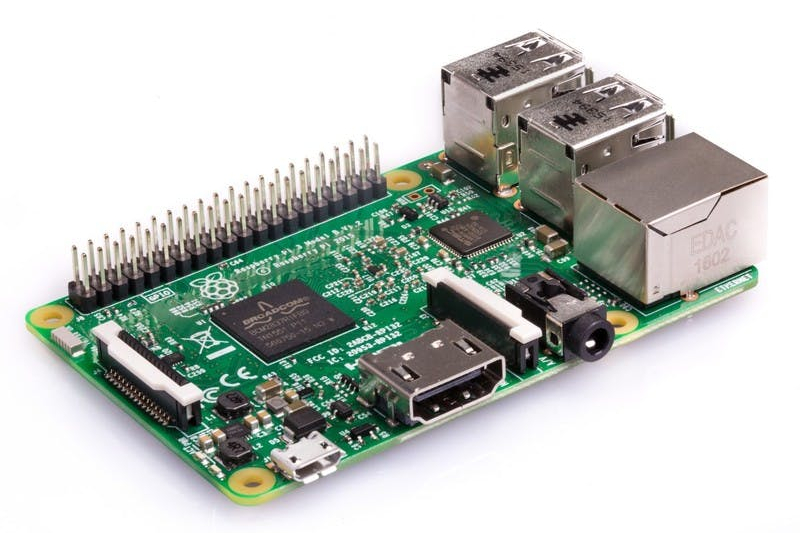
\includegraphics[width=\textwidth/2]{raspberry_pi_3b}
                \caption{Raspberry Pi 3B \cite{imagen_raspberry_pi_3b}\label{fig:ImagenRaspberryPi3B}}
            \end{figure}

            Se ha vuelto un producto tan popular que se vende para todo tipo de usos, desde centros
            multimedia \cite{centro_multimedia_raspberry_pi} o espejos inteligentes \cite{espejo_raspberry_pi}, hasta
            respiradores \cite{github_respirador} o este mismo proyecto.

        % subsection ¿Qué es Raspberry Pi? (end)

        \subsection{Modelos} % (fold)
        \label{sub:ModelosRaspberryPi}

            En sus ocho años de existencia, la Fundación Raspberry Pi ha lanzado cinco modelos de la Raspberry Pi, con
            diferentes variaciones. En la figura \ref{fig:ImagenModelosPi} se detallan alguno de los detalles de estos
            modelos \cite{raspberry_pi_wikipedia_en}:

            \begin{figure}[ht]
                \centering
                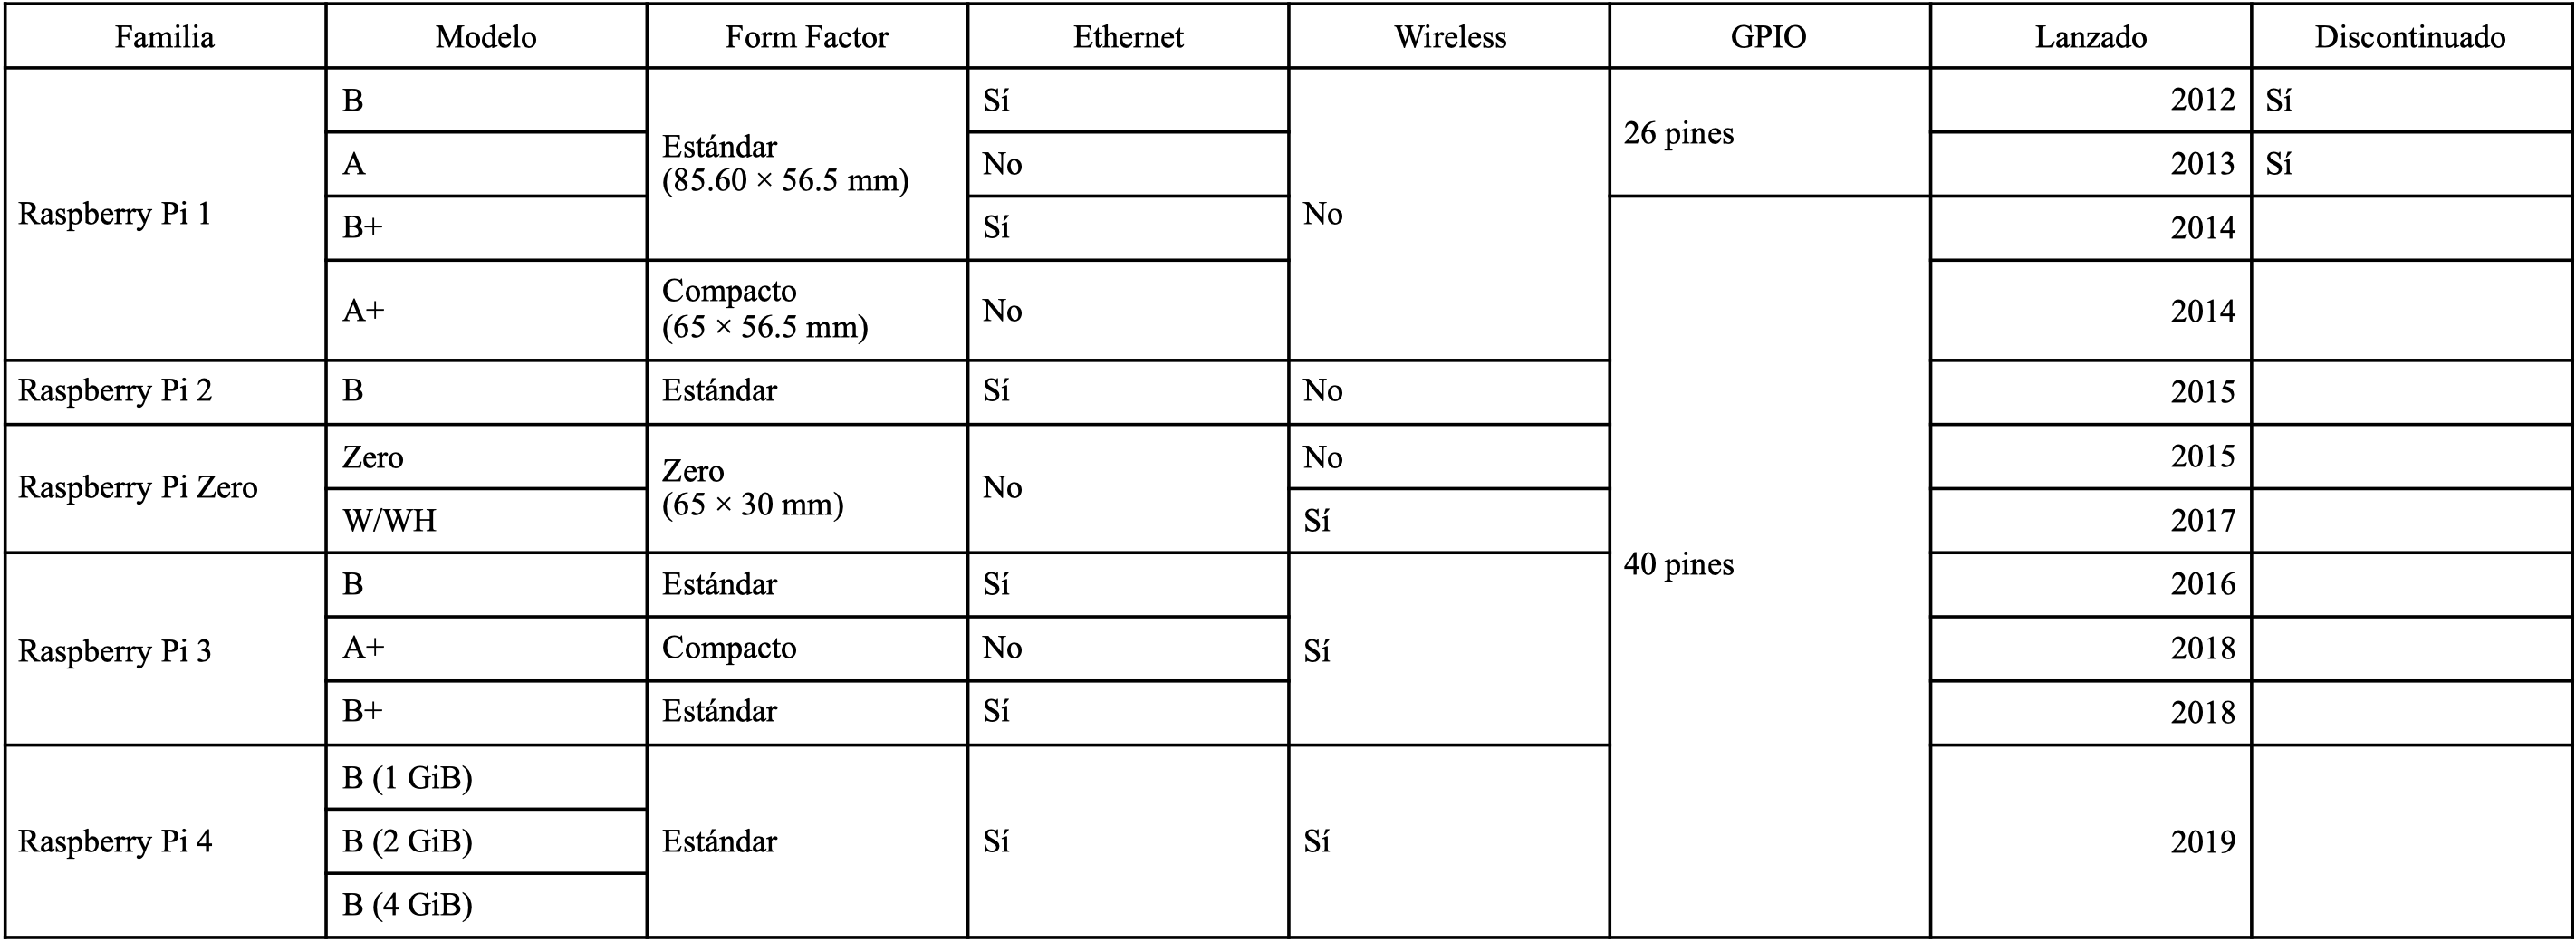
\includegraphics[width=\textwidth]{tabla_modelos_raspberry_pi}
                \caption{Tabla modelos de Raspberry Pi \cite{raspberry_pi_wikipedia_en}\label{fig:ImagenModelosPi}}
            \end{figure}

        % subsection Modelos (end)

        \subsection{Hardware} % (fold)
        \label{sub:HardwareRaspberryPi}

            La Raspberry Pi 3B utilizada en este proyecto tiene el siguiente hardware \cite{raspberry_pi_hardware}:

            \begin{itemize}
                \item \textbf{Procesador:} Broadcom BCM2837 de cuatro núcleos con arquitectura ARM Cortex A53 (ARMv8) a
                1.2 GHz.
                \item \textbf{Memoria:} 1GB de memoria LPDDR2
                \item \textbf{GPU:} Broadcom VideoCore IV a 250 MHz
                \item \textbf{USB:} Cuatro puertos USB 2.0.
                \item \textbf{GPIO:} Hay 40 pines de GPIO (General Purpose Input/Output). Estos pines funcionan a 3.3V.
                \item \textbf{Internet:} Ethernet 10/100 Mbit/s y WiFi 802.11 b/g/n
            \end{itemize}

        % subsection Hardware (end)

        \subsection{Alternativas} % (fold)
        \label{sub:AlternativasRaspberryPi}

            Podemos encontrar una gran variedad de alternativas, algunas de ellas son las
            siguientes \cite{alternativas_raspberry_pi}:

            \begin{itemize}
                \item \textbf{Orange Pi Prime}: Esta alternativa está viendo un gran crecimiento en los últimos años. La
                compañía que la fabrica se centra en precios más baratos y una gran personalización de la placa.
                \item \textbf{Banana Pi M3}: Puede compararse en prestaciones con la Raspberry Pi 3, sin embargo, el
                precio es mayor, ya que esta cuesta alrededor de \$80
                \item \textbf{ ASUS Tinker Board}: Es la más compatible a nivel de software, además, cuenta con más
                potencia de cálculo, lo que reduce los tiempos de procesamiento.
                \item \textbf{Huawei HiKey 960}: La alternativa de Huawei es la que cuenta con más potencia. Utiliza el
                procesador que utilizan los teléfonos de la compañía (Kirin 960). Pero también es la más cara, \$300.
            \end{itemize}

            Tras ver estas alternativas, se ha decidido utilizar la Raspberry Pi, principalmente, por ser la estándar
            entre las placas. Es la que más documentación tiene en Internet, haciendo, por tanto, más sencillo el
            desarrollo del proyecto y, al ser la más utilizada, también es más sencillo hacerse con ella desde
            España.

            En concreto, se utiiza el modelo Raspberry Pi 3B, por ser el modelo más avanzado en el momento de la compra,
            aunque un mes después se lanzó la Raspberry Pi 4, con mayor potencia y memoria, entre otras cosas.

        % subsection Alternativas (end)

        \subsection{Lucha contra el Covid-19} % (fold)
        \label{sub:LuchaContraElCovid-19}

            Debido a la reciente crisis del coronavirus Covid-19, muchas personas empezaron a utilizar la Raspberry Pi
            para ayudar a luchar contra el virus. La principal utilidad que se encontró para esta placa en esa situación
            fue la de crear respiradores, pudiendo usar un código publicado en Github \cite{github_respirador} para
            programar la Raspberry Pi.

            Las ventas, por tanto, se dispararon, llegando a las 640.000 unidades vendidas en el mes de
            marzo \cite{ventas_raspberry_pi_covid}.

        % subsection Lucha contra el Covid-19 (end)

    % section Raspberry Pi (end)

    \section{Arduino} % (fold)
    \label{sec:Arduino}

        \subsection{¿Qué es Arduino?} % (fold)
        \label{sub:QueEsArduino}

            ``Arduino es una plataforma electrónica de código abierto basada en hardware y software fácil de usar. Las
            placas Arduino pueden leer entradas (luz en un sensor, un dedo en un botón o un mensaje de Twitter) y
            convertirlo en una salida: activar un motor, encender un LED, publicar algo online. Para hacerlo, utiliza
            el lenguaje de programación Arduino y el Software Arduino (IDE).''

            \begin{flushright}
                (Arduino, 2 de abril de 2020. \cite{arduino_introduction})
            \end{flushright}

            El proyecto Arduino nació en el año 2003 en el Interaction Design Institute Ivrea en Italia y, tanto la
            placa como el software que utiliza son open-source.

            \begin{figure}[ht]
                \centering
                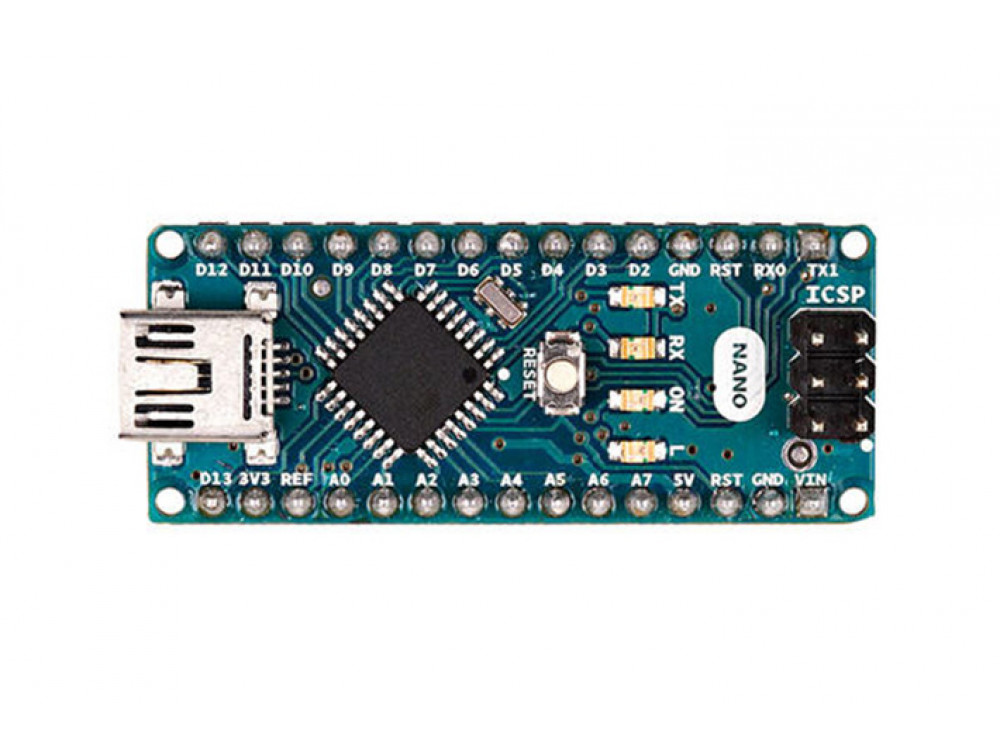
\includegraphics[width=\textwidth/2]{arduino_nano}
                \caption{Arduino Nano \cite{imagen_arduino_nano}\label{fig:ImagenArduinoNano}}
            \end{figure}

        % subsection ¿Qué es Arduino? (end)

        \subsection{Modelos} % (fold)
        \label{sub:ModelosArduino}

            En la figura \ref{fig:ImagenModelosArduino} se especifican los modelos de entrada de Arduino junto con
            algunas de sus especificaciones de hardware \cite{arduino_compare}:

            \begin{figure}[ht]
                \centering
                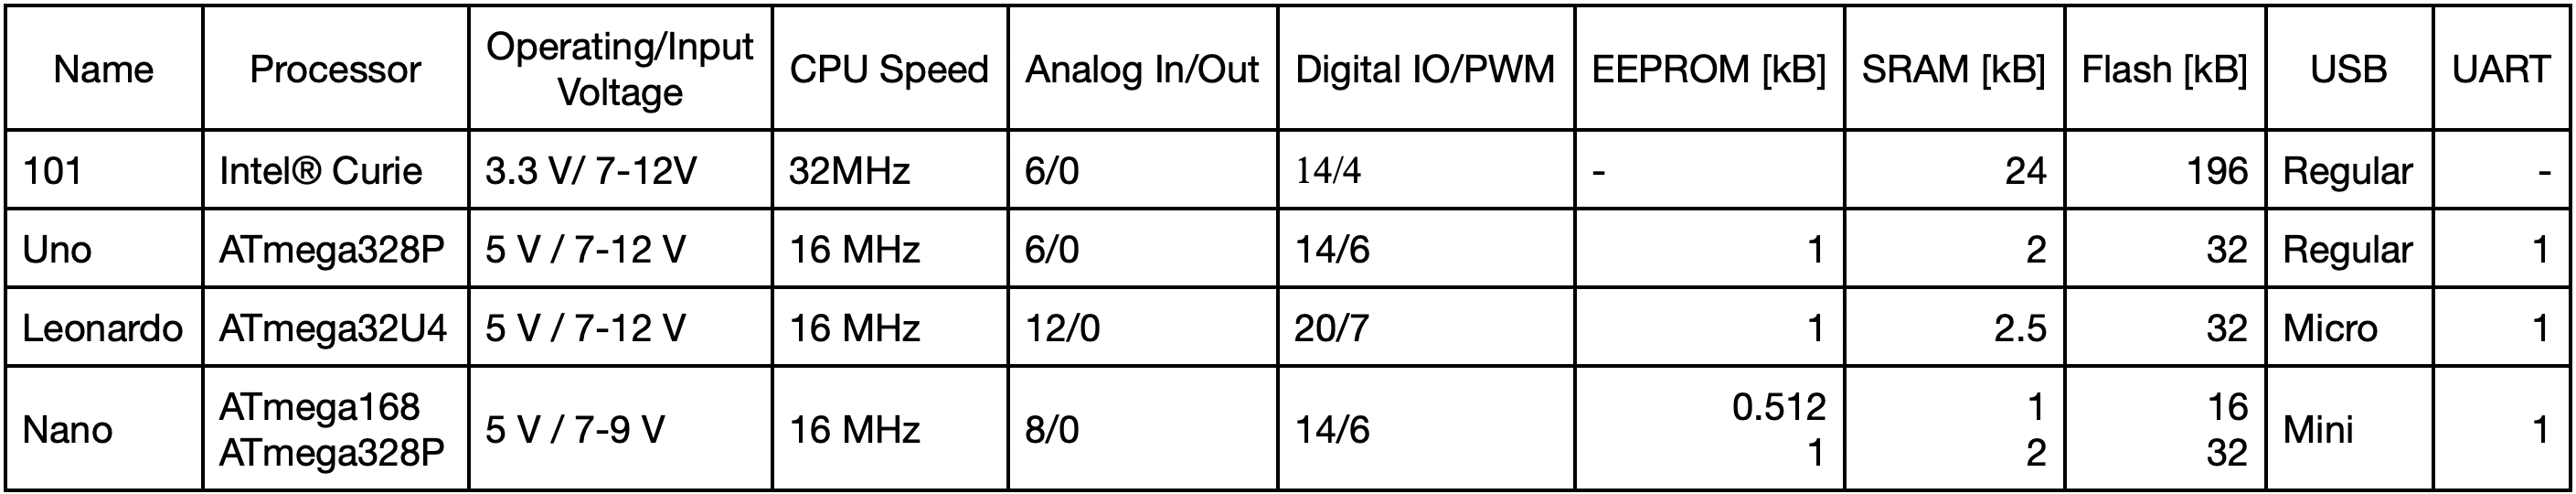
\includegraphics[width=\textwidth]{tabla_modelos_arduino}
                \caption{Tabla modelos de Arduino \cite{arduino_compare}\label{fig:ImagenModelosArduino}}
            \end{figure}

            El modelo utilizado en este proyecto es el Arduino Nano.

        % subsection Modelos (end)

        \subsection{Alternativas} % (fold)
        \label{sub:AlternativasArduino}

            Al igual que para Raspberry Pi (\ref{sub:AlternativasRaspberryPi}), hay una gran variedad de alternativas
            para la placa Arduino \cite{alternativas_arduino}:

            \begin{itemize}
                \item \textbf{NodeMCU}: Es la solución más barata. Además, añade la posibilidad de ejecutar código Lua.
                \item \textbf{Teensy 3}: Esta placa incluye un procesador más potente, haciéndola capaz de ejecutar
                tareas más pesadas. También se puede programar mediante el Arduino IDE, con la biblioteca Teensyduino.
                \item \textbf{MSP430 Launchpad}: Esta alternativa se centra en un consumo de energía más bajo que la
                Arduino.
            \end{itemize}

            Arduino, al igual que Raspberry Pi, es la estándar en este tipo de placas y cuenta con una mayor
            documentación y ejemplos disponibles. En concreto se utiliza el modelo Arduino Nano, que es uno de los
            modelos más pequeños de la placa, con potencia suficiente para este proyecto.

        % subsection Alternativas (end)

    % section Arduino (end)

    \section{Opciones actuales en el mercado} % (fold)
    \label{sec:OpcionesActualesEnElMercado}

        Son múltiples las baterías electrónicas a la venta. Una búsqueda rápida en Thomann \cite{thomann_baterias} nos
        muestra una gran variedad de baterías electrónicas en un amplío rango de precios, desde los 109\euro{} hasta los
        8.398\euro{}.

        \begin{figure}[ht]
            \centering
            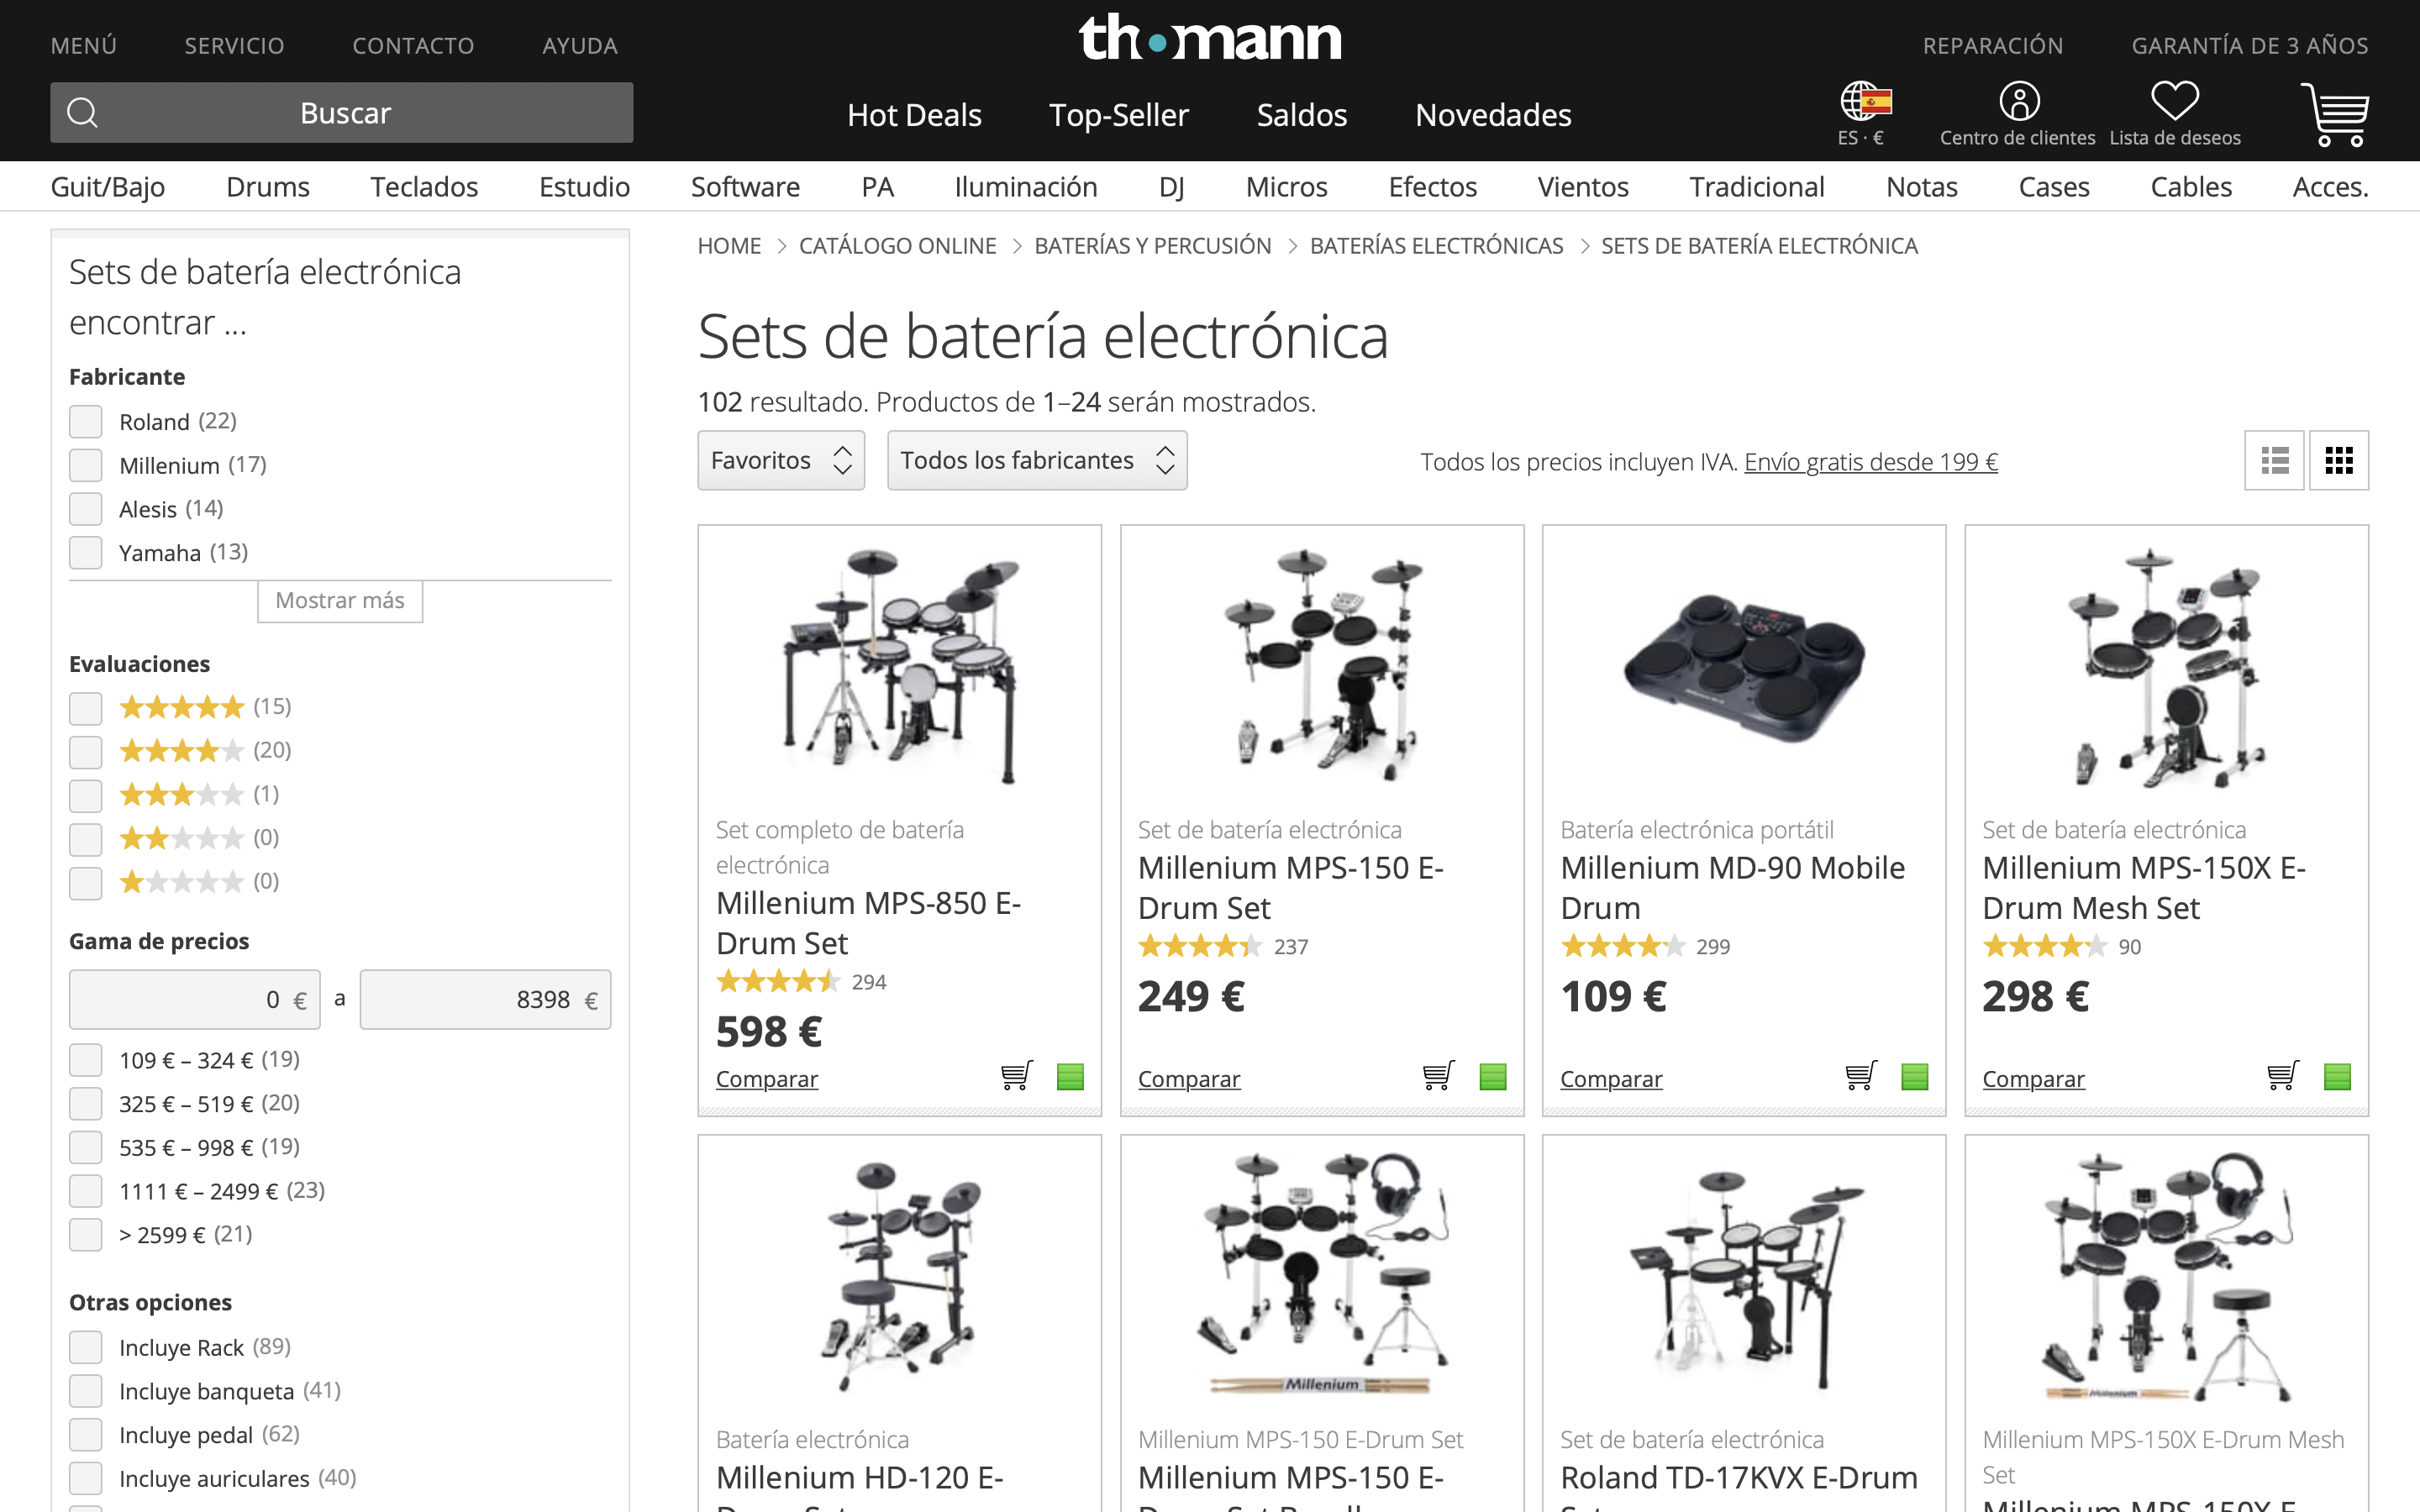
\includegraphics[width=\textwidth]{thomann_baterias}
            \caption{Resultados de la búsqueda de baterías electrónicas en Thomann \cite{thomann_baterias}
                     \label{fig:ThomannBusqueda}}
        \end{figure}

        En el terreno de las baterías que los usuarios se pueden construir (DIY), los principales resultados
        \cite{drum_magazine_diy_kit} utilizan elementos como sensores piezoeléctricos y sintetizadores MIDI. Los precios
        de estos sintetizadores van desde 150\euro{} a 2100\euro{}.

    % section Opciones actuales en el mercado (end)

    \section{Propuesta} % (fold)
    \label{sec:Propuesta}

        La propuesta que se presenta es un crear un programa de código abierto para que cualquier persona con unos
        conocimiento medios de informática pueda montar su propia batería electrónica en casa.

        Para completar con éxito el objetivo de este proyecto, los puntos más importantes serán:

        \begin{itemize}
            \item Reproducción del sonido con el menor delay posible.
            \item Reproducción de varios sonidos de manera concurrente.
            \item Sensación de tocar la batería lo más realista posible.
        \end{itemize}

    % section Propuesta (end)

% chapter Estado del arte (end)


%%%%%%%%%%%%%%%%%%%%%%%%%%%%%%%%%%%%%%%%%%%%%%%%%%%%%%%%%%%%%%%%%%%%%%%%%%%%%%%%%
% Aspectos legales
%%%%%%%%%%%%%%%%%%%%%%%%%%%%%%%%%%%%%%%%%%%%%%%%%%%%%%%%%%%%%%%%%%%%%%%%%%%%%%%%%

\chapter{Aspectos legales} % (fold)
\label{cha:AspectosLegales}

    \section{Derechos de autor} % (fold)
    \label{sec:DerechosDeAutor}
        \subsection{¿Qué son los derechos de autor?} % (fold)
        \label{sub:QueSonLosDerechosDeAutor}

            Los derechos de autor son una serie de leyes que protegen la autoría de las obras. Estas pueden ser libros,
            películas, obras de teatro, programas informáticos...

            Se cubren dos tipos de derechos: los derechos patrimoniales, que aseguran que el autor obtenga compensación
            financiera, y los derechos morales, que cubren todo lo que no esté relacionado con los derechos
            patrimoniales, por ejemplo, la prohibición de que se modifique la obra \cite{derechos_ompi}.

        % section ¿Qué son los derechos de autor? (end)

        \subsection{Historia de los derechos de autor} % (fold)
        \label{sub:HistoriaDeLosDerechosDeAutor}

            La historia de los derechos de autor comienza en 1710, cuando se publica el Estatuto de la Reina
            Anna \cite{estatuto_anna} que fue el primer reglamento sobre los derechos de autor. En el momento de la
            publicación de éste estatuto solo se contemplaban los derechos sobre los libros, pero en posteriores leyes
            se contemplan otros usos, como cine, radio, fotografías o programas de ordenador.

            En la actualidad, los derechos de autor se protegen tanto con acuerdos y leyes internacionales, como leyes
            nacionales.

            Desde 1974 en Estados Unidos con la CONTU \cite{contu} (Commission on New Technological Uses of Copyrighted
            Works) y de 1991 en la Unión Europea con la Computer Programs Directive \cite{com_pro_dir}, se protegen los
            derechos de autor de los programas informáticos.

        % subsection Historia de los derechos de autor (end)

        \subsection{Derechos de autor en España} % (fold)
        \label{sub:DerechosDeAutorEnEspana}

            En España tenemos la Ley de Propiedad Intelectual. En esta ley, la propiedad intelectual se define como:

            ``La obra literaria, artística o científica, expresadas en cualquier medio (libros, escritos, composiciones
            musicales, obras, coreografías, obras audiovisuales, esculturas, obras pictóricas, planos, maquetas, mapas,
            fotografías, programas de ordenador y bases de datos) que corresponde a su autor por el solo hecho de su
            creación, que tiene derecho a explotarla y disponer de ella a su voluntad.''

            \begin{flushright}
                (La Ley de Propiedad Intelectual y los derechos de autor en España. \cite{propiedad_intelectual_espana})
            \end{flushright}

            \subsubsection{Tipos de derechos} % (fold)
            \label{ssub:TiposDeDerechos}

                En la Ley de Propiedad Intelectual se definen dos grupos de derechos de autor:

                \begin{itemize}
                    \item \textbf{Derechos morales}: Corresponden al autor de la obra y no se puede renunciar a ellos ni
                    traspasarlos. Se encargan de proteger la identidad y reputación del autor.
                    \item \textbf{Derechos patrimoniales}: Estos sí se pueden traspasar. Sirven para que el autor decida
                    cómo se utiliza y representa su obra. No se puede usar la obra sin autorización expresa.
                \end{itemize}
            
            % subsubsection Tipos de derechos (end)

            \subsubsection{Programas de ordenador} % (fold)
            \label{ssub:ProgramasDeOrdenador}

                La Ley de Propiedad Intelectual define \textit{programa de ordenador} como:

                ``A los efectos de la presente Ley se entenderá por programa de ordenador toda secuencia de
                instrucciones o indicaciones destinadas a ser utilizadas, directa o indirectamente, en un sistema
                informático para realizar una función o una tarea o para obtener un resultado determinado, cualquiera
                que fuere su forma de expresión y fijación.

                A los mismos efectos, la expresión programas de ordenador comprenderá también su documentación
                preparatoria. La documentación técnica y los manuales de uso de un programa gozarán de la misma
                protección que este Título dispensa a los programas de ordenador.''

                \begin{flushright}
                    (Real Decreto Legislativo 1/1996, de 12 de abril. \cite{prop_intelectual})
                \end{flushright}

                El autor del programa será la persona o grupo de personas que lo hayan creado y tendrán derechos de
                explotación sobre el programa durante la vida del autor y setenta años después de su muerte.

                El autor tendrá derecho a realizar o autorizar:

                \begin{itemize}
                    \item Reproducicción total o parcial.
                    \item Traducción, adaptación, arreglo o cualquier cambio.
                    \item Distribución pública.
                \end{itemize}
            
            % subsubsection Programas de ordenador (end)
        
        % subsection Derechos de autor en España (end)
    
    % section Derechos de autor (end)

    \section{Origen de sonidos de batería} % (fold)
    \label{sec:OrigenDeSonidosDeBateria}

        Los sonidos de batería han sido obtenidos de la biblioteca de sonidos de GarageBand para macOS \cite{garageband}.
        Estos sonidos son libres y gratuitos para usarse composiciones musicales o proyectos de audio originales, tal y
        como estipula la página oficial de Apple \cite{support_garageband}.

    % section Origen de sonidos de batería (end)

% chapter Aspectos legales (end)

\newpage


%%%%%%%%%%%%%%%%%%%%%%%%%%%%%%%%%%%%%%%%%%%%%%%%%%%%%%%%%%%%%%%%%%%%%%%%%%%%%%%%%
% Diseño
%%%%%%%%%%%%%%%%%%%%%%%%%%%%%%%%%%%%%%%%%%%%%%%%%%%%%%%%%%%%%%%%%%%%%%%%%%%%%%%%%

\chapter{Diseño de la propuesta} % (fold)
\label{cha:Diseno}

    %% Aquí hay que detallar y justificar las decisiones que se tomen (hacer varias propuestas pero desarrollar solo la
    %% mejor) (siempre es bueno una tabla comparativa con pros y contras o ticks)

    \section{Tecnologías empleadas} % (fold)
    \label{sec:TecnologiasEmpleadas}

        \subsection{C} % (fold)
        \label{sub:CLanguage}

            El lenguaje utilizado para la mayor parte del proyecto ha sido C. C es un lenguaje desarrollado en 1972 por
            Dennis Ritchie en los Laboratios Bell. Fue creado para la creación de sistemas operativos, como UNIX, y es
            muy valorado por su eficiencia.

            En la actualidad, es uno de los lenguajes más populares. Está disponible en muchas plataformas, desde
            superordenadores, hasta sistemas empotrados. Fue diseñado para mapear las instrucciones escritas en C a
            lenguaje máquina de forma muy eficiente, con pocas instrucciones, esto hace que sea muy eficiente en
            cualquier plataforma en la que se utilice.\cite{wikipedia_c_language}

            Es por esta eficiencia, por la que se ha utilizado en el proyecto. Cualquier instrumento musical, y en
            especial una batería, requiere que las acciones realizadas por el músico tengan una reacción rápida por el
            sistema, y C puede proporcionar esta velocidad.

        % subsection C (end)

        \subsection{Visual Studio Code} % (fold)
        \label{sub:VisualStudioCode}

            Visual Studio Code es un editor de texto diseñado por Microsoft para Windows, Linux y macOS, lanzado al
            público en 2016.

            Su sencillez, compatibilidad con una gran cantidad de lenguajes de programación y una extensa biblioteca de
            extensiones han hecho que VS Code sea uno de los editores de texto más populares entre los programadores.
            \cite{wikipedia_vs_code}

            \begin{figure}[ht]
                \centering
                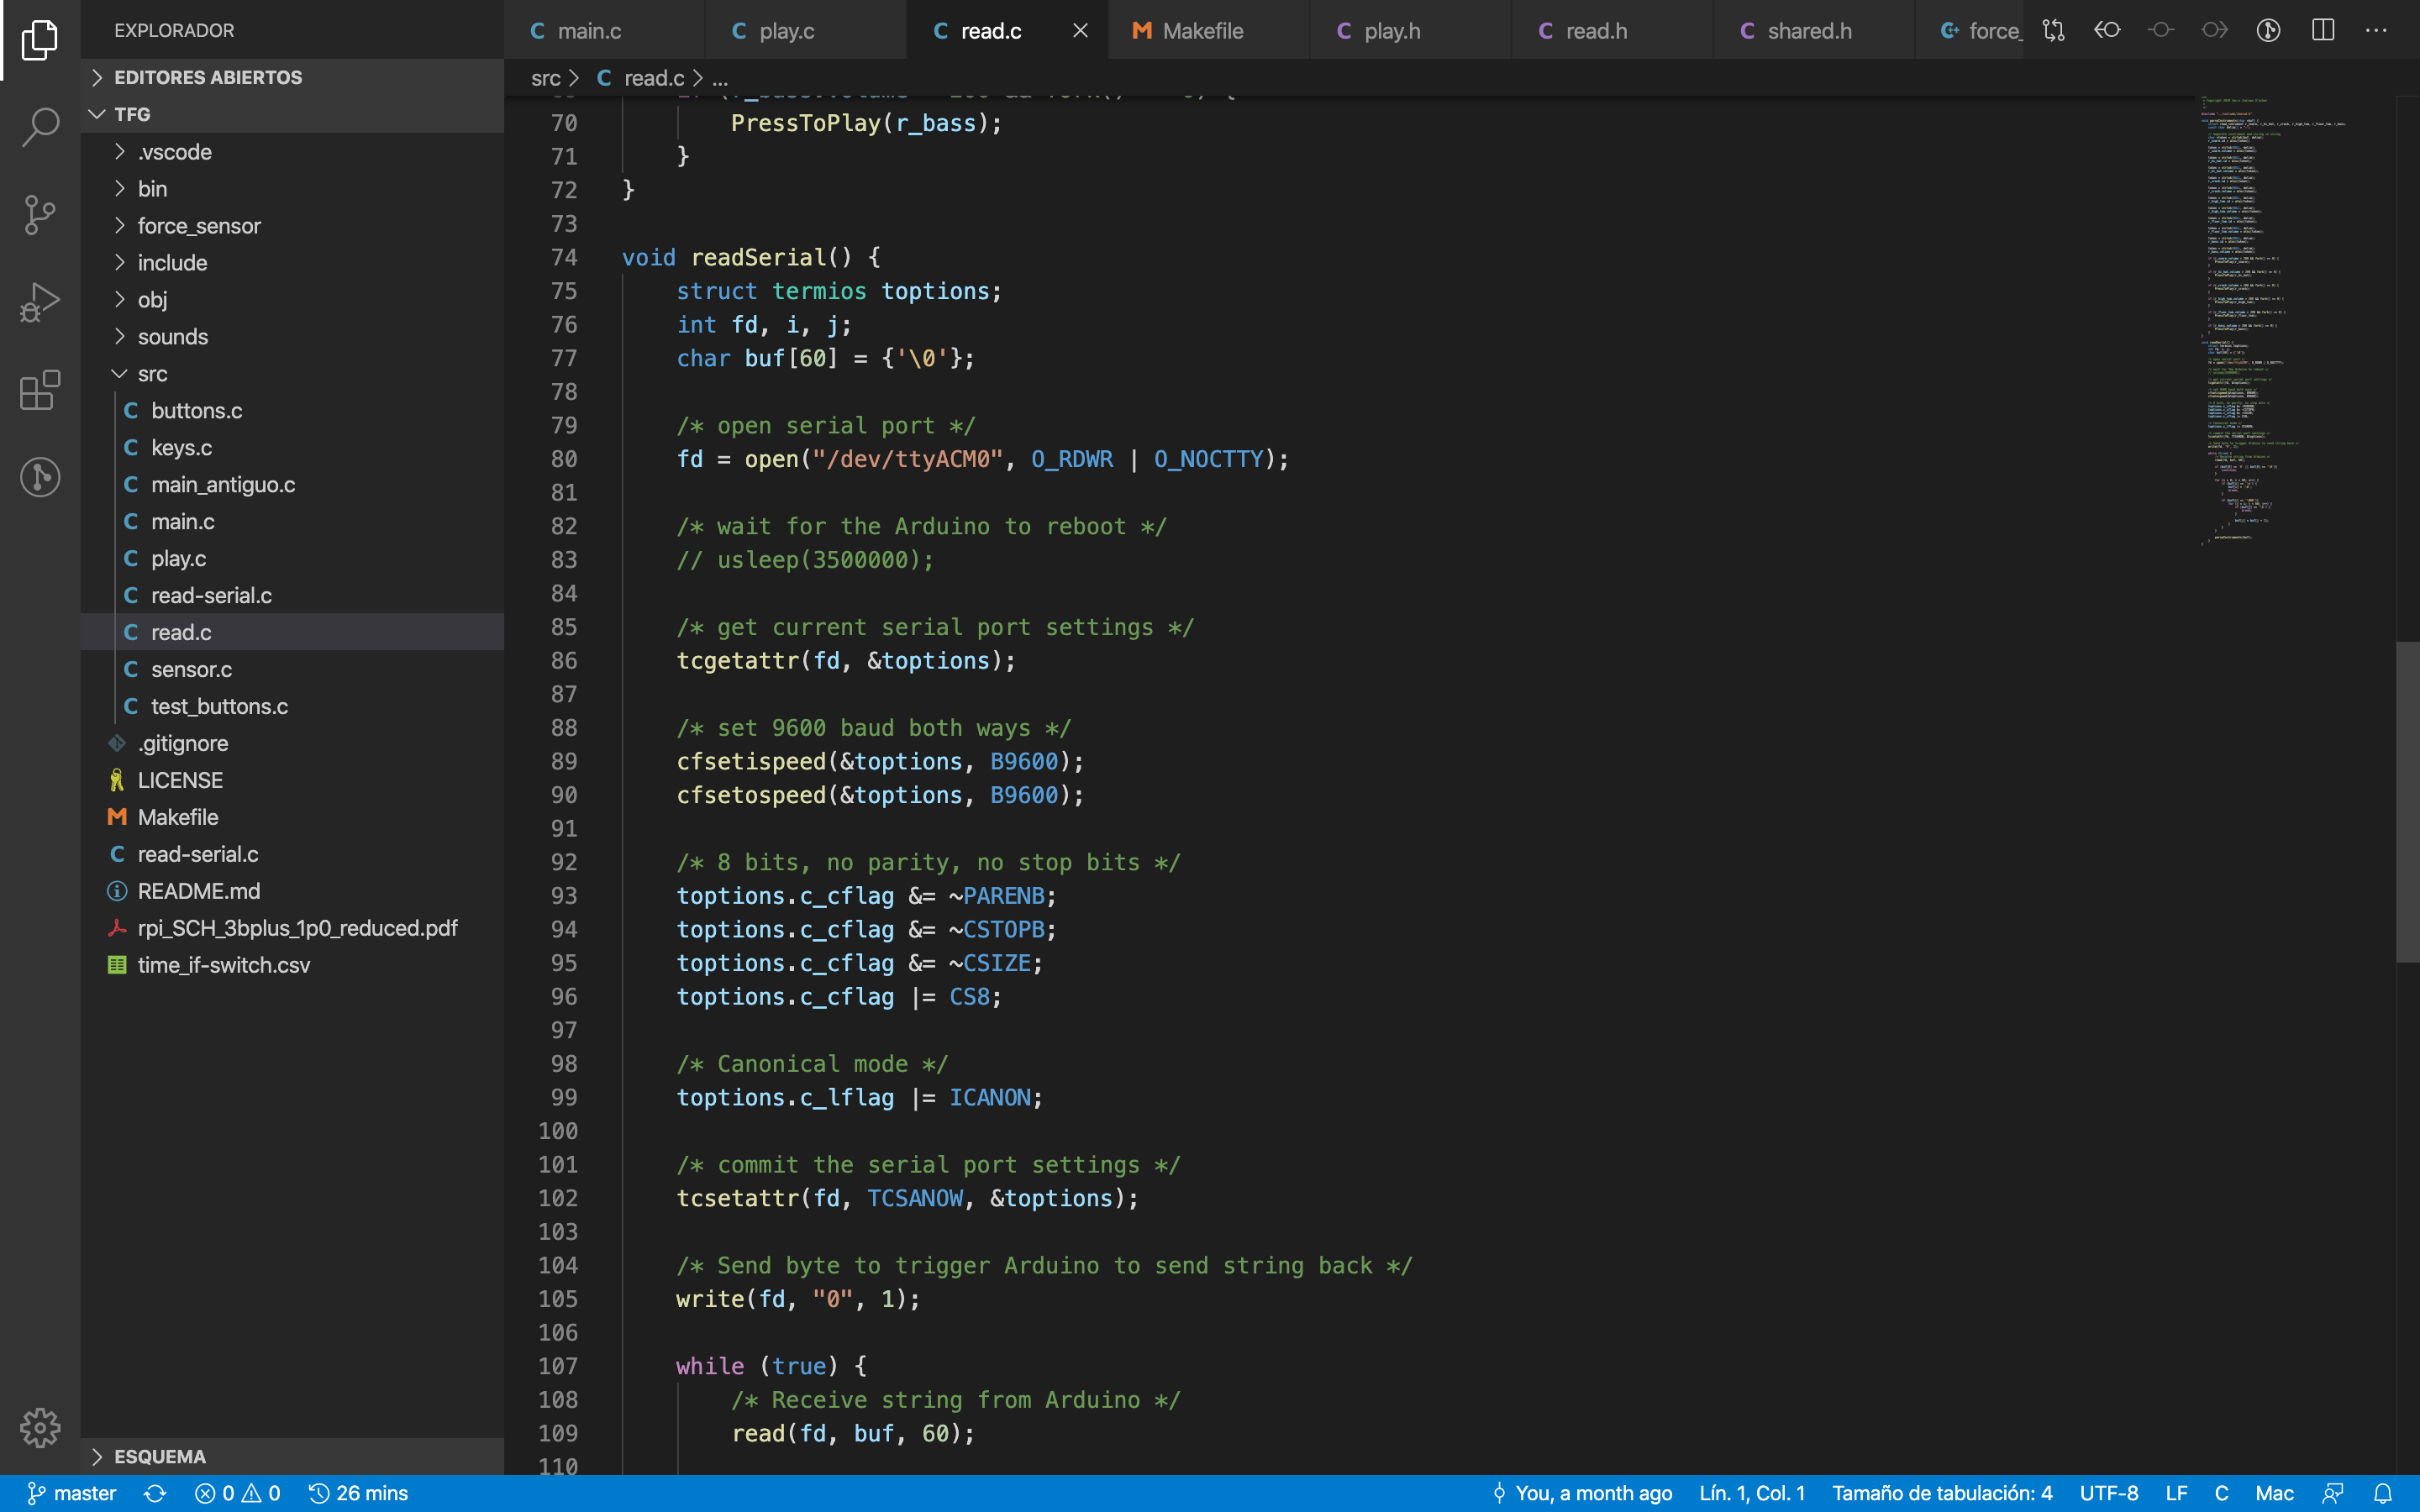
\includegraphics[width=\textwidth]{vs_code}
                \caption{Captura de pantalla de Visual Studio Code \label{fig:VisualStudioCode}}
            \end{figure}

            \newpage

        % subsection Visual Studio Code (end)

        \subsection{Github} % (fold)
        \label{sub:Github}

            Github es un servicio de alojamiento de código abierto y control de versiones mediante Git.

            En este proyecto se ha utilizado principalmente para llevar ese control de versiones del código y para
            organizar los diferentes pasos a dar y los errores encontrados durante el desarrollo mediante su capacidad
            de crear \textit{issue}. Aparte, Github permite que este código esté disponible para el acceso de cualquier
            persona y que cualquiera pueda contribuir a él.

            \begin{figure}[ht]
                \centering
                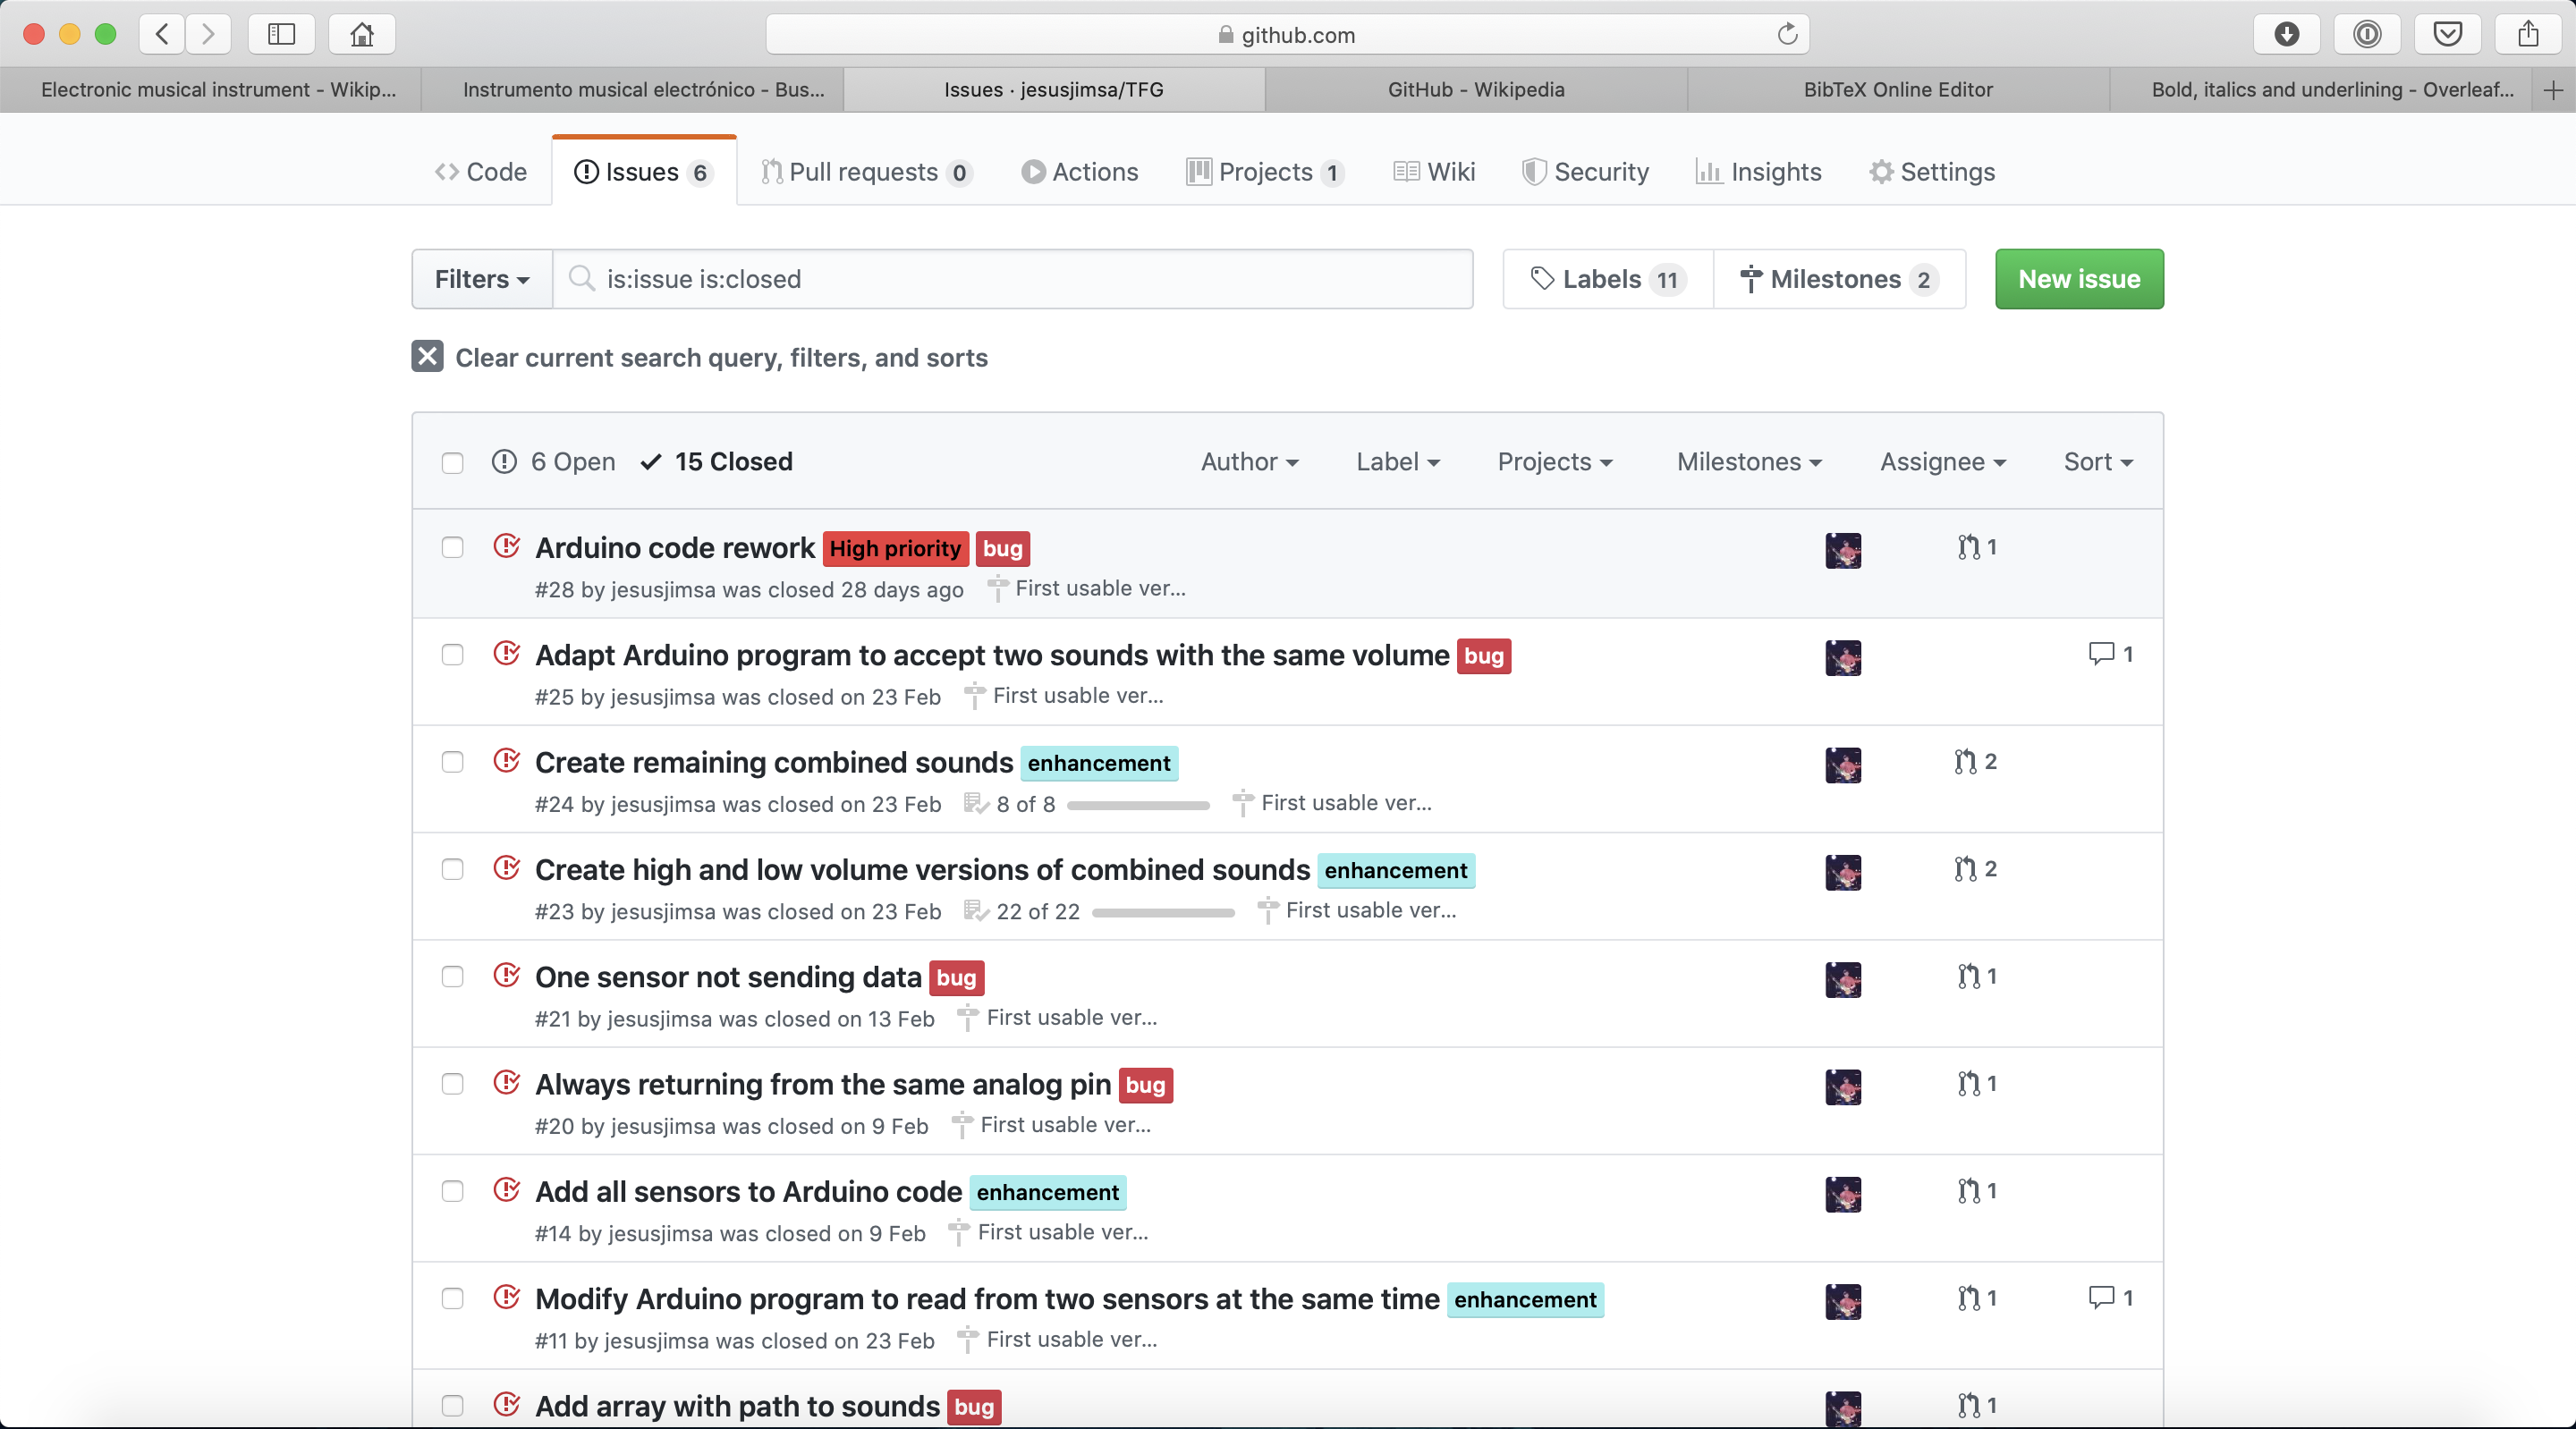
\includegraphics[width=\textwidth]{github_issues}
                \caption{Captura de pantalla de las issues de Github del proyecto \label{fig:GithubIssues}}
            \end{figure}

            \newpage

        % subsection Github (end)

        \subsection{Clockify} % (fold)
        \label{sub:Clockify}

            Clockify es una aplicación de seguimiento de tiempo. Ha sido utilizada para llevar un seguimiento de cuánto
            tiempo ha sido dedicado a la creación y desarrollo de este proyecto y su memoria.

            \begin{figure}[ht]
                \centering
                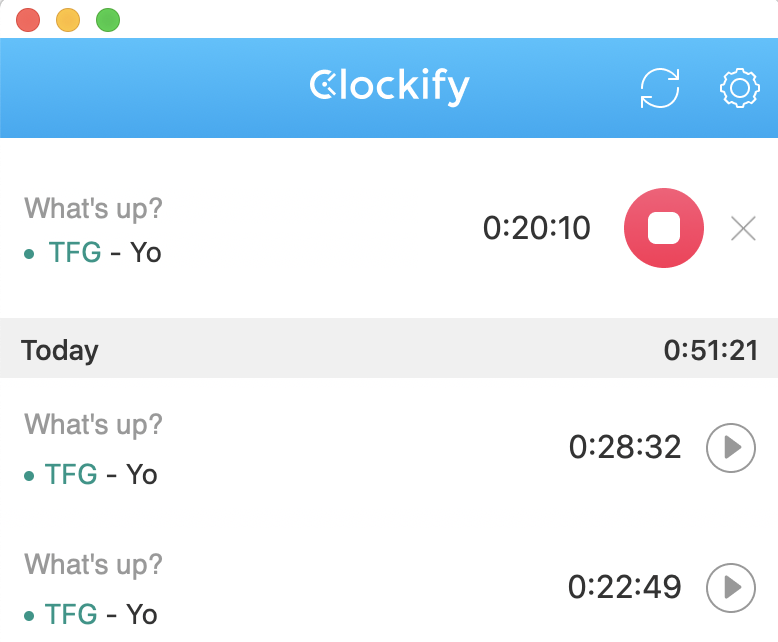
\includegraphics[width=\textwidth/2]{clockify}
                \caption{Captura de pantalla de Clockify \label{fig:ClockifyCaptura}}
            \end{figure}

        % subsection Clockify (end)

        \subsection{Overleaf} % (fold)
        \label{sub:Overleaf}

            Overleaf es un editor de LaTeX online y colaborativo. Permite crear documentos en LaTeX y la colaboración de
            hasta dos personas en su modalidad gratuita.

            En este proyecto, ha facilitado la compartición de esta memoria entre alumno y tutor para su corrección, a
            parte de servir como editor principal de LaTeX.

            \begin{figure}[ht]
                \centering
                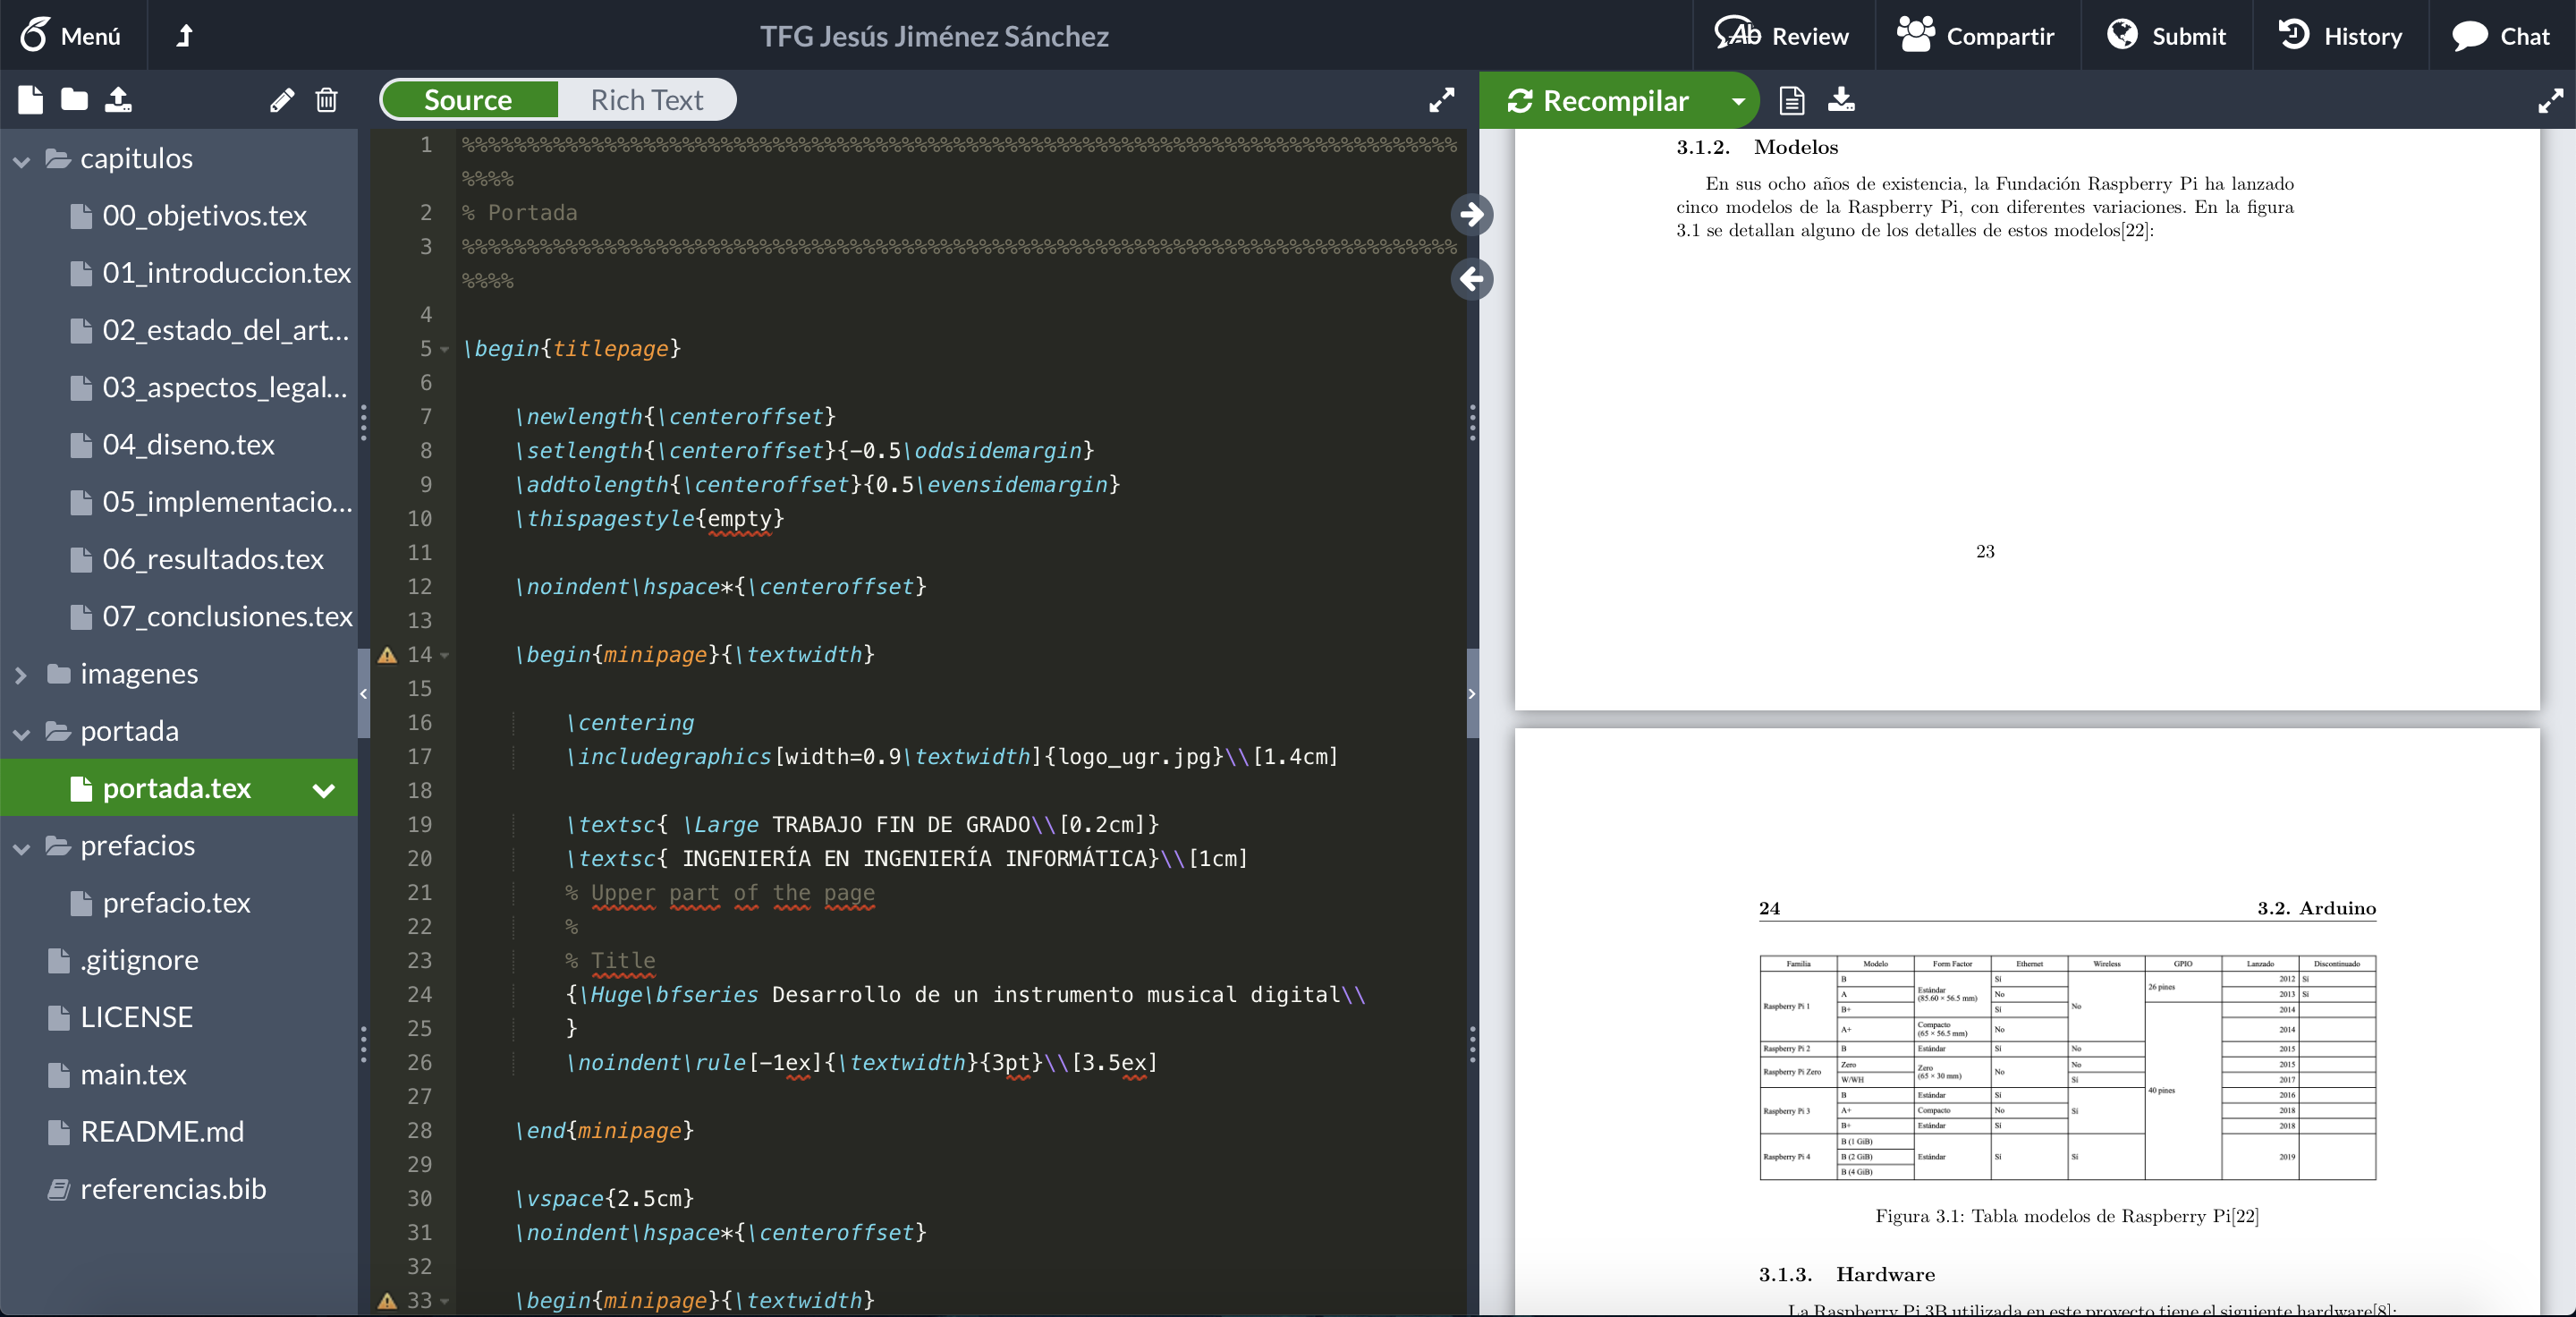
\includegraphics[width=\textwidth]{captura_overleaf}
                \caption{Captura de pantalla de Overleaf \label{fig:OverleafCaptura}}
            \end{figure}

        % subsection Overleaf (end)

    % section Tecnologías empleadas (end)

    \section{Decisiones tomadas} % (fold)
    \label{sec:DecisionesTomadas}

        La primera decisión fue entre hacer detección binaria de la entrada, es decir, si el parche ha sido golpeado o
        no, y hacer que estas entradas sean concurrentes (al golpear dos parches, el sonido de ambos suena al mismo
        tiempo), o hacer detección de distintos sonidos en un mismo parche, dependiendo de cómo se golpee el parche (en
        el centro, en el lateral, con más o menos fuerza…) el sonido emitido es diferente.\newline

        Se decide empezar con la primera alternativa y dejar la segunda para más adelante, en caso de tener tiempo.

        \subsection{Librería de reproducción de sonido} % (fold)
        \label{sub:LibreriaDeReproduccionDeSonido}

            \subsubsection{playsound} % (fold)
            \label{ssub:Playsound}

                Al principio se comenzó buscando implementar el proyecto en Python, por ser un lenguaje sencillo y con
                gran variedad de librerías. Sin embargo, tras probar playsound\cite{playsound}, la librería de
                reproducción de sonidos más popular de Python, se decidió que era muy lenta, y en este proyecto, la
                velocidad a la que se reproducen los sonidos es primordial. Por esta razón, se descarta playsound.

            % subsubsection playsound (end)

            \subsubsection{mpg123} % (fold)
            \label{ssub:Mpg123}

                Mpg123\cite{mpg123} es una librería y programa en C más rápido que playsound de Python. Tiene el problema de
                hacer que haya fallos de memoria cuando se usan hebras para reproducir varios sonidos al mismo tiempo, pero
                se soluciona utilizando procesos en su lugar.

            % subsubsection mpg123 (end)

            \subsubsection{libao} % (fold)
            \label{ssub:Libao}

                Esta librería se usa en conjunto con mpg123 para reproducir el sonido de la batería.
                mpg123 es la encargada de descodificar el archivo mp3 que contiene el sonido, mientras que
                libao\cite{libao} utiliza la información que obtiene mpg123 y manda la señal al sistema operativo para
                reproducir el audio.

            % subsubsection libao (end)

        % subsection Librería de reproducción de sonido (end)

        \subsection{Otras librerías} % (fold)
        \label{sub:OtrasLibrerias}

            \begin{itemize}
                \item
                Wiring Pi\cite{wiringPi}: Para realizar la conexión de sensores y botones a la Raspberry Pi se utiliza
                la librería wiringPi, que es la estándar en este tema. Esta librería se ha utilizado unicamente en los
                prototipos, ya que al principio se pretendía realizar el proyecto enteramente en la Raspberry Pi, pero
                finalmente se ha utilizado una Arduino para realizar la lectura de sensores.
            \end{itemize}

        % subsection Otras librerías (end)

        \subsection{if-else vs switch} % (fold)
        \label{sub:if-else_vs_switch}

            Al pulsar una tecla, el número leído se envía a una función que selecciona qué sonido hay que reproducir en
            ese momento, dependiendo de qué sonido corresponda a ese número. Este proceso de selección se puede hacer
            con una estructura de \textit{if-else} anidados o con un \textit{switch-case}.\newline

            Para decidir cuál de las dos soluciones se implementa en la versión final se realizó un test en el que cada
            vez se ejecutan más iteraciones del programa cambiando de sonido en cada una de ellas. Se empieza con 1
            iteración y se termina con 10000000 iteraciones.\newline

            \begin{figure}[ht]
                \centering
                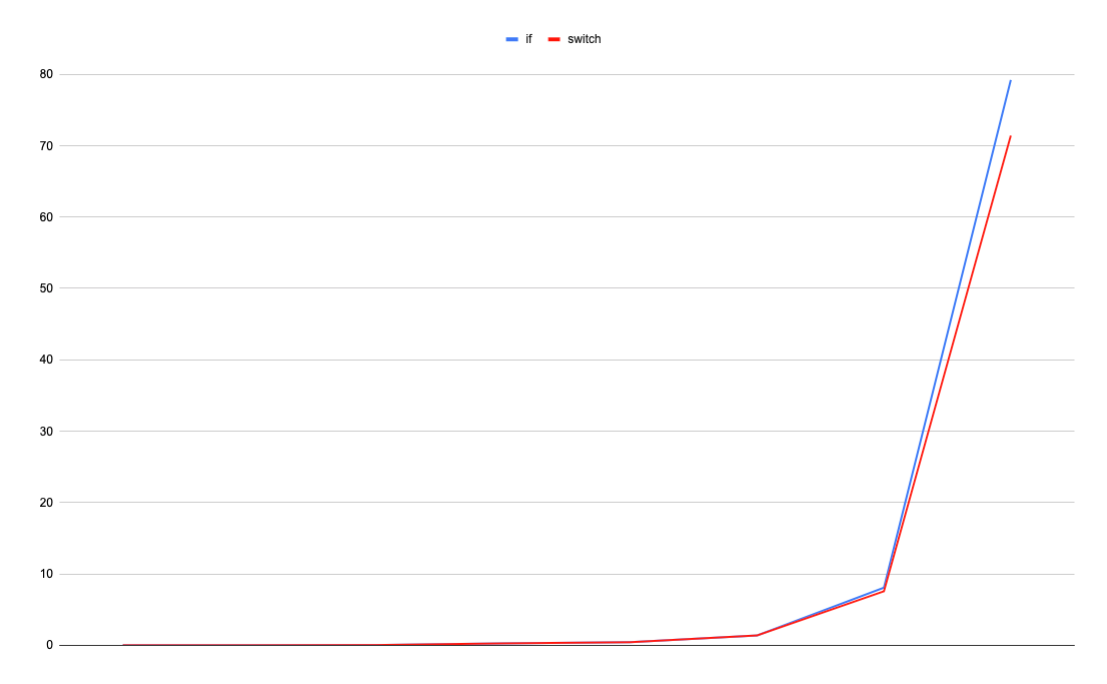
\includegraphics[width=\textwidth]{grafica_if_switch}
                \caption{Gráfica comparativa if-else vs switch \label{fig:GraficaIfVsSwitch}}
            \end{figure}

            \begin{center}
                \begin{tabular}{ |c|c|c| }
                    \hline
                        iterations & if & switch \\
                        \hline\hline
                        1 & 0.000243 & 0.000270 \\
                        \hline
                        10 & 0.002797 & 0.002485 \\
                        \hline
                        100 & 0.027775 & 0.027261 \\
                        \hline
                        1000 & 0.260075 & 0.261464 \\
                        \hline
                        10000 & 0.431544 & 0.425668 \\
                        \hline
                        100000 & 1.368561 & 1.374575 \\
                        \hline
                        1000000 & 8.070825 & 7.560718 \\
                        \hline
                        10000000 & 79.199539 & 71.409653 \\
                    \hline
                \end{tabular}
            \end{center}

            Como se puede ver en la figura \ref{fig:GraficaIfVsSwitch}, la diferencia no es apreciable hasta las
            1000000 iteraciones, pero después pasa a casi 8 segundos de diferencia en 10000000 iteraciones. Por
            esta razón se ha decidido que la función utilice la estructura \textit{switch-case}.\newline

            Finalmente, debido a la manera en la que realizan las comprobaciones de qué botones y sensores son
            utilizados, aunque un \textit{switch-case} es más rápido, esta estructura se reserva para la versión del
            programa que reproduce los sonidos leyendo del teclado. En el programa que controla los sensores se
            utiliza una estructura \textit{if-else}.

        % subsection if-else vs switch (end)

    % section Decisiones tomadas (end)

    \section{Arduino vs Raspberry Pi} % (fold)
    \label{sec:ArduinoVsRaspberryPi}

        Para la recepción de las señales de los sensores de presión RP c18.3 y RP S40, se plantean dos opciones, se
        puede utilizar la propia Raspberry Pi en la que se ejecuta el programa que maneja los sonidos o una Arduino
        Nano. En el proyecto resultante se utiliza finalmente la Arduino debido a dos razones principales.\newline

        La primera razón es el precio y la escalabilidad, una Raspberry Pi cuesta 39,95\euro{} mientras que una
        Arduino Nano cuesta 10\euro{}. Una Arduino Nano cuenta con menos pines de E/S, pero añadir una placa es más
        barato y sencillo que añadir una placa de Raspberry Pi.\newline

        La segunda razón es la implementación del programa que se encarga de el sensor de presión. En Internet se
        pueden encontrar ejemplos y tutoriales refiriéndose a cómo implementar el sistema en una Arduino, pero no
        es tan fácil encontrar información para hacerlo desde una Raspberry Pi.\newline

        Por estas razones se elige realizar la recepción de las señales del sensor de presión desde la Arduino,
        haciendo el proceso más sencillo y más barato.

        \subsection{Conexión} % (fold)
        \label{sub:Conexion}

            Para realizar la conexión de los sensores se utilizan cables de protoboard conectados de la forma
            explicada en la figura \ref{fig:EsquemaConexion}:

            \begin{figure}[ht]
                \centering
                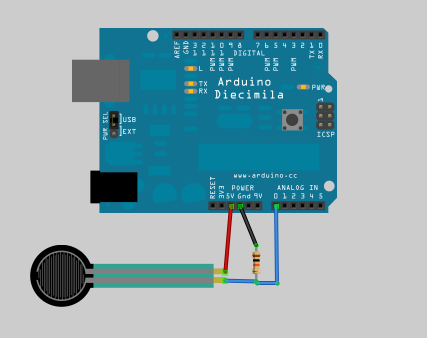
\includegraphics[width=\textwidth]{force_sensor_arduino}
                \caption{Esquema de conexión de sensores de presión\cite{force_sensor_arduino}
                         \label{fig:EsquemaConexion}}
            \end{figure}

        % subsection Conexión (end)

    % section Arduino vs Raspberry Pi (end)

% chapter Diseño (end)

\newpage


%%%%%%%%%%%%%%%%%%%%%%%%%%%%%%%%%%%%%%%%%%%%%%%%%%%%%%%%%%%%%%%%%%%%%%%%%%%%%%%%%
% Implementación
%%%%%%%%%%%%%%%%%%%%%%%%%%%%%%%%%%%%%%%%%%%%%%%%%%%%%%%%%%%%%%%%%%%%%%%%%%%%%%%%%

\chapter{Implementación de la propuesta}
\label{cha:Implementacion}

    Este capítulo está dedicado a la explicación de cómo se ha desarrollado el proyecto. Se detalla la forma en la que
    se reproduce el sonido y cómo se hace de forma paralela, se explican los principales problemas encontrados en el
    desarrollo y se comenta el presupuesto y el tiempo empleado.

    \section{Reproducción de sonido} % (fold)
    \label{sec:ReproduccionDeSonido}

        La reproducción del sonido se realiza utilizando las dos bibliotecas mencionadas en el capítulo
        anterior \ref{sub:LibreriaDeReproduccionDeSonido}, mpg123 y libao.

        El proceso completo que se sigue desde que se pulsa uno de los sensores hasta que se reproduce el sonido es el
        siguiente:
        \begin{enumerate}
            \item Uno de los sensores de presión realiza una lectura y manda el valor leído a la placa Arduino.
            \item El Arduino, prepara un mensaje que escribe en el log del monitor serie (\ref{sec:SonidoEnParalelo}).
            \item La función \texttt{readSerial} lee de \textit{/dev/ttyACM0}, la salida del monitor serie, filtra que
            no sea un mensaje vacío o de que no hay que reproducir nada y se manda a parsear.
            \item En \texttt{parseInstruments} se procesa el mensaje leído.
            \item En la función \texttt{PressToPlay} se selecciona qué instrumento debe sonar.
            \item Finalmente, en la función \texttt{play}, se descodifica el archivo de sonido correspondiente y se
            reproduce utilizando las dos bibliotecas anteriormente mencionadas.
        \end{enumerate}

        El flujo del programa es el representado en la figura \ref{fig:DiagramaFlujo}:

        \newpage

        \begin{figure}[ht]
            \centering
            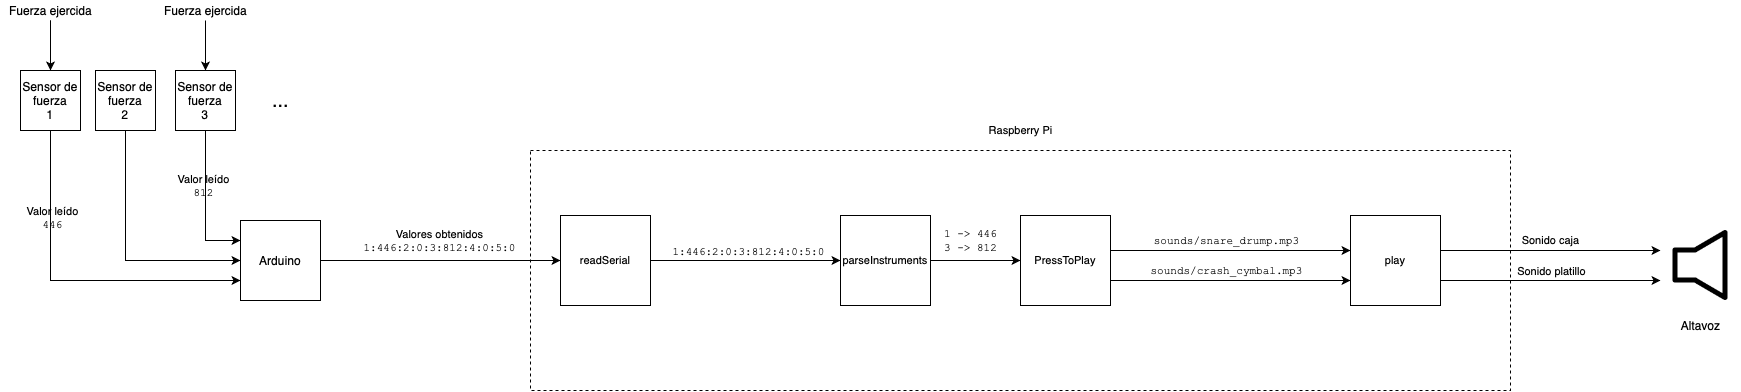
\includegraphics[width=\textwidth]{diagrama_flujo}
            \caption{Diagrama de flujo\label{fig:DiagramaFlujo}}
        \end{figure}

    % section Reproducción de sonido (end)

    \section{Sonido en paralelo} % (fold)
    \label{sec:SonidoEnParalelo}

        Hasta febrero, todas las versiones del programa fueron diseñadas pensando solo en emitir un sonido cada vez,
        pero lo preferible en un proyecto como este es que se emita más de un sonido al mismo tiempo.

        El primer acercamiento fue mediante un sistema de máximos y sonidos combinados. En esta primera solución, se
        escogía el mayor de los seis sonidos y, si había un segundo sonido con un valor mayor que 200 (el mínimo para
        emitir sonido), se enviaba un mensaje a través del log de Arduino seleccionando un sonido combinado. Estos
        sonidos habían sido combinados previamente utilizando los sonidos ya presentes en el proyecto.

        Finalmente, esta solución no funcionó correctamente (no se enviaba la señal del sonido combinado) y se procedió
        a diseñar una nueva. Esta nueva solución es la que se utiliza actualmente en el proyecto. Consiste en mandar
        todas las señales al mismo tiempo. Antes de la implementación de esta solución, el log era así:

        \begin{verbatim}
        0:0
        0:0
        2:364
        0:0
        0:0
        \end{verbatim}

        En este mensaje, se indica que el pad 2 registra una presión de intensidad 364 (sobre 1023). Los \texttt{0:0}
        indican que ningún pad registra presión.

        Tras la implementación de la solución, el log es así:

        \begin{verbatim}
        0:0
        0:0
        1:446:2:0:3:812:4:0:5:0
        0:0
        0:0
        1:0:2:0:3:0:4:902:5:0
        0:0
        \end{verbatim}

        En estos mensajes se envía la siguiente información:

        \begin{enumerate}
            \item Los mensajes de \texttt{0:0} indican que ningún pad registra presión.
            \item El primer mensaje indica que se han tocado:
            \begin{itemize}
                \item El pad 1 con intensidad 446
                \item El pad 2 no registra presión
                \item El pad 3 con intensidad 812
                \item El pad 4 no registra presión
                \item El pad 5 no registra presión
            \end{itemize}
            \item El segundo mensaje indica que se han tocado:
            \begin{itemize}
                \item El pad 1 no registra presión
                \item El pad 2 no registra presión
                \item El pad 3 no registra presión
                \item El pad 4 con intensidad 902
                \item El pad 5 no registra presión
            \end{itemize}
        \end{enumerate}

        En cuanto un sensor detecta una presión mayor a 200, se manda el mensaje de todos los sensores al mismo tiempo.
        En caso de que el valor leído sea menor que 200, se manda como 0, pero si es mayor, se manda con los demás. Este
        mensaje es leído y procesado por la Raspberry Pi, que lanzará los procesos necesarios con los sonidos que hagan
        falta según los sensores que hayan sido presionados.

        Con esta segunda propuesta, el programa envía correctamente la señal de todos los sensores y los sonidos son
        emitidos correctamente.

    % section Sonido en paralelo (end)

    \section{Principales problemas} % (fold)
    \label{sec:PrincipalesProblemas}

        \subsection{Número de lecturas en botones} % (fold)
        \label{sub:NumeroDeLecturasEnBotones}

            En el prototipo con botones, al pulsar o dejar pulsado un botón, el programa reproduciría el mismo
            sonido muchas veces. Para solucionar esto se crea una hebra por cada botón, cuando se pulsa, entrará
            en un bucle infinito del que no saldrá hasta que el botón no sea soltado. Al usarse hebras, nos
            permite pulsar más botones al mismo tiempo.

        % subsection Número de lecturas en botones (end)

        \subsection{Hebras vs procesos} % (fold)
        \label{sub:HebrasVSProcesos}

            La primera aproximación a cómo realizar este proyecto fue usando hebras POSIX para lanzar los sonidos al
            mismo tiempo, por ser más ligeras, en cuanto a uso de recursos, que los procesos lanzados por \texttt{fork}.
            Sin embargo, debido a la implementación de biblioteca utilizada para reproducir sonidos, al lanzar estas
            hebras para reproducir varios sonidos al mismo tiempo, se producía un error de \textit{segmentation fault}.
            La solución a este problema fue sustituir las hebras POSIX por procesos generados por la llamada a
            \texttt{fork()}.

        % subsection Hebras vs procesos (end)

        \subsection{Número de lecturas en sensores} % (fold)
        \label{sub:NumeroDeLecturasEnSensores}

            El sensor de presión devuelve muchas lecturas por segundo. Para solucionar esto a la hora de reproducir los
            sonidos hay dos formas de solucionarlo: una es introduciendo un \textit{delay} lo suficientemente grande
            para diferenciar dos toques del sensor, la otra solución, que ha sido la implementada, trata de bloquear el
            sensor cada vez que se entra en uno de los tres intervalos de volumen que se han elegido. Cada vez que entra
            en uno de estos intervalos de deja de leer hasta que no baje la presión lo suficiente. Si la presión sube,
            tampoco enviará señal para que reproduzca sonido.

        % subsection Número de lecturas en sensores (end)

        \subsection{Construcción de paths} % (fold)
        \label{sub:ConstruccionDePaths}

            Al añadir el sensor y el Arduino, el programa que controlaba los sonidos emitidos recibía las mediciones
            del Arduino y, dependiendo de los datos entregados por éste, se emite un sonido a un volumen concreto.
            La construcción de la cadena de texto que contenía el \textit{path} se hacía mediante las funciones de
            copia y concatenación \textit{strcat} y \textit{strdup}. El problema es que al recibir el \textit{path},
            la biblioteca de reproducción de sonidos lanzaba el siguiente error:

            \begin{verbatim}
            malloc(): corrupted top size
            make: *** [Makefile:19: run] Segmentation fault
            \end{verbatim}

            Tras muchas pruebas, como aumentar la cantidad de memoria reservada para el \textit{path} o para el
            buffer que se utiliza en la función de reproducción, o probar a que siempre se enviara el mismo path,
            sin leer del Arduino (reproduciendo el sonido satisfactoriamente), finalmente se decide cambiar la forma en
            la que se genera el path, \textit{hardcodeándolo} en el programa. Esto resulta funcionar y es la solución
            que ha sido implementada en el programa.

        % subsection Construcción de paths (end)

    % section Principales problemas (end)

    \section{Pads} % (fold)
    \label{sec:Pads}

        Los pads son las superficies que son golpeadas para generar los sonidos. Para este proyecto se han fabricado
        usando madera, cola y gomaeva \cite{GomaEva}. El coste total de fabricar un pad es de 1,54\euro{}. Comparado
        con otros productos similares como los de Prologix \cite{practice_pad}, cuyo kit de práctica de 4 pads cuesta
        \$224,99, el precio de la solución propuesta en este proyecto es sensiblemente inferior.

        \subsection{Madera MDF} % (fold)
        \label{sub:MaderaMDF}

            La madera utilizada para fabricar los pads es de tipo MDF. Este tipo de madera se refiere a tableros
            fabricados utilizando fibras de madera y resinas sintéticas para aportar una mayor
            resistencia \cite{mdf_santana}.

            \begin{figure}[ht]
                \centering
                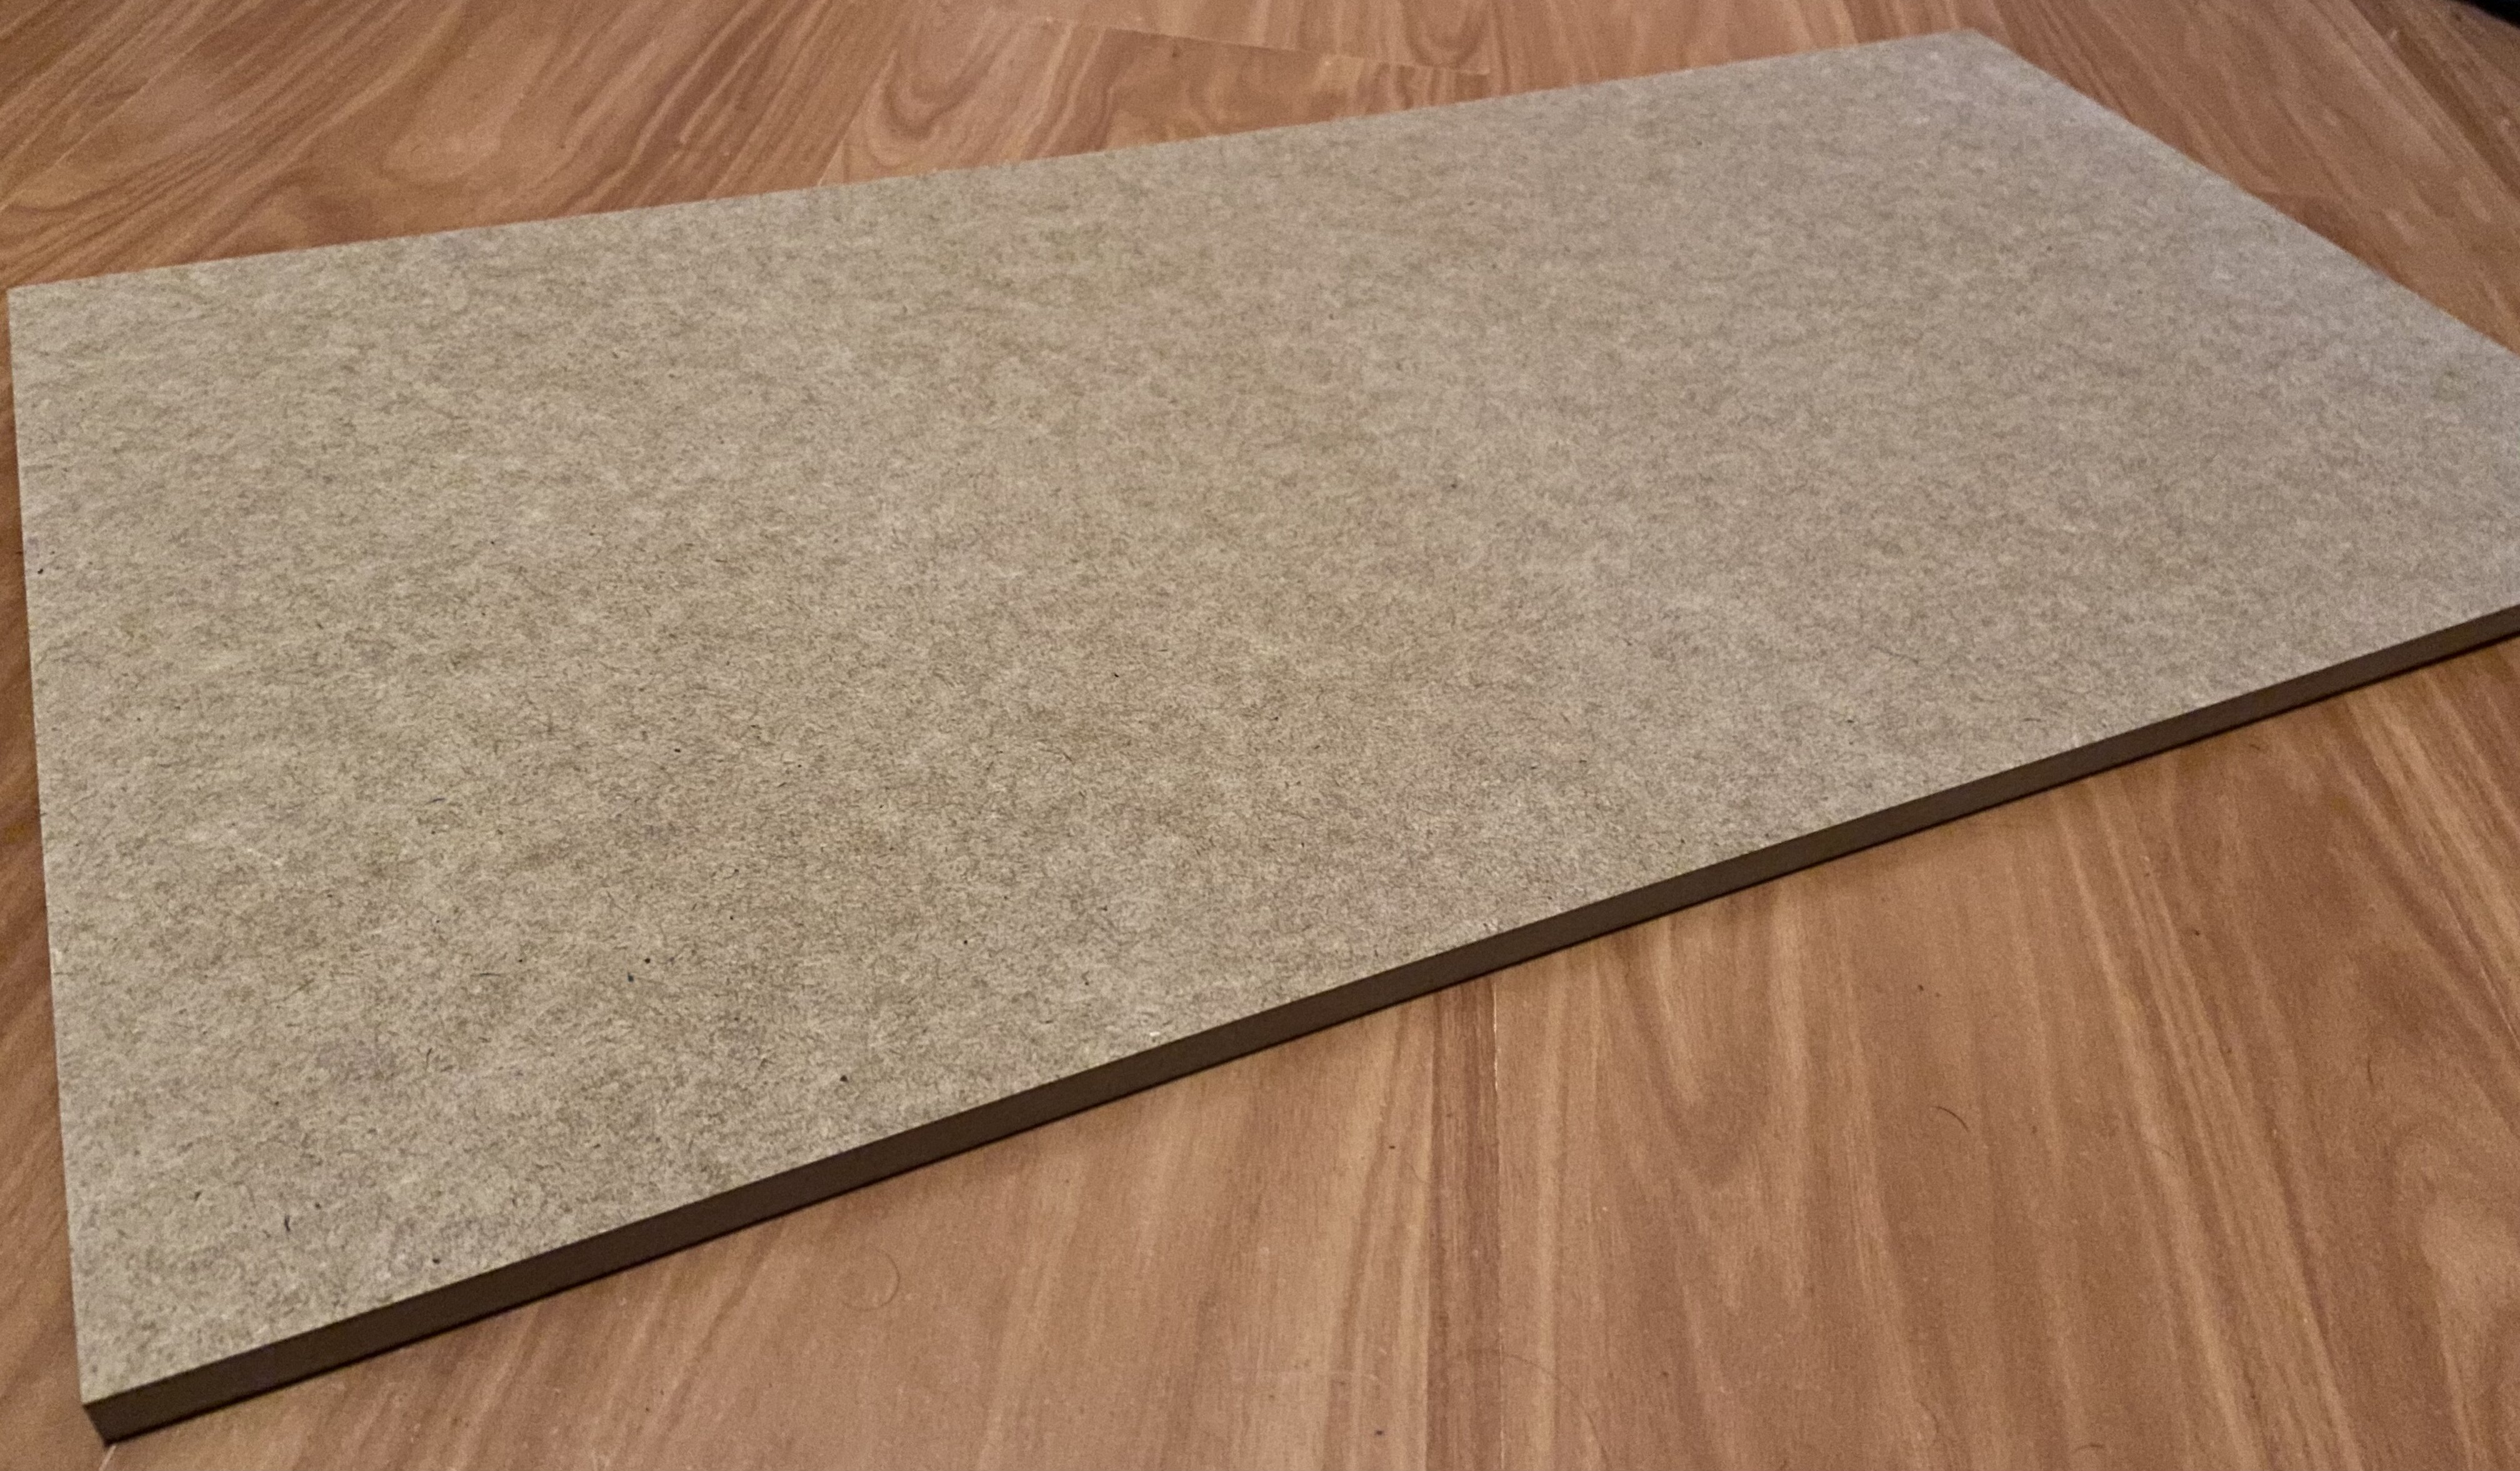
\includegraphics[width=\textwidth]{tablero_mdf}
                \caption{Imagen de tablero MDF\label{fig:TableroMDF}}
            \end{figure}

        % subsection Madera MDF (end)

        \subsection{Construcción} % (fold)
        \label{sub:ConstruccionPads}

            Los pads están hechos a partir de un tablero de madera MDF de 600x300x10 mm. Este tablero se cortó en un
            principio en dos círculos de unos 20 cm de diámetro, con la intención de tener unos sensores de fuerza lo
            suficientemente grandes como para tener sensibilidad de la mayor parte de estos pads. Sin embargo, los
            sensores que finalmente se han usado en el proyecto son más pequeños de lo esperado inicialmente, de
            4x5,5 cm. Debido a esto, se tuvieron que recortar nuevos pads más pequeños, para que los sensores cubrieran
            la mayor area del pad posible. Estos nuevos pads contaban con unos 12 cm de diámetro. El resultado después
            de recortarlos es el indicado en la figura \ref{fig:PadsRecortados}.

            \begin{figure}[ht]
                \centering
                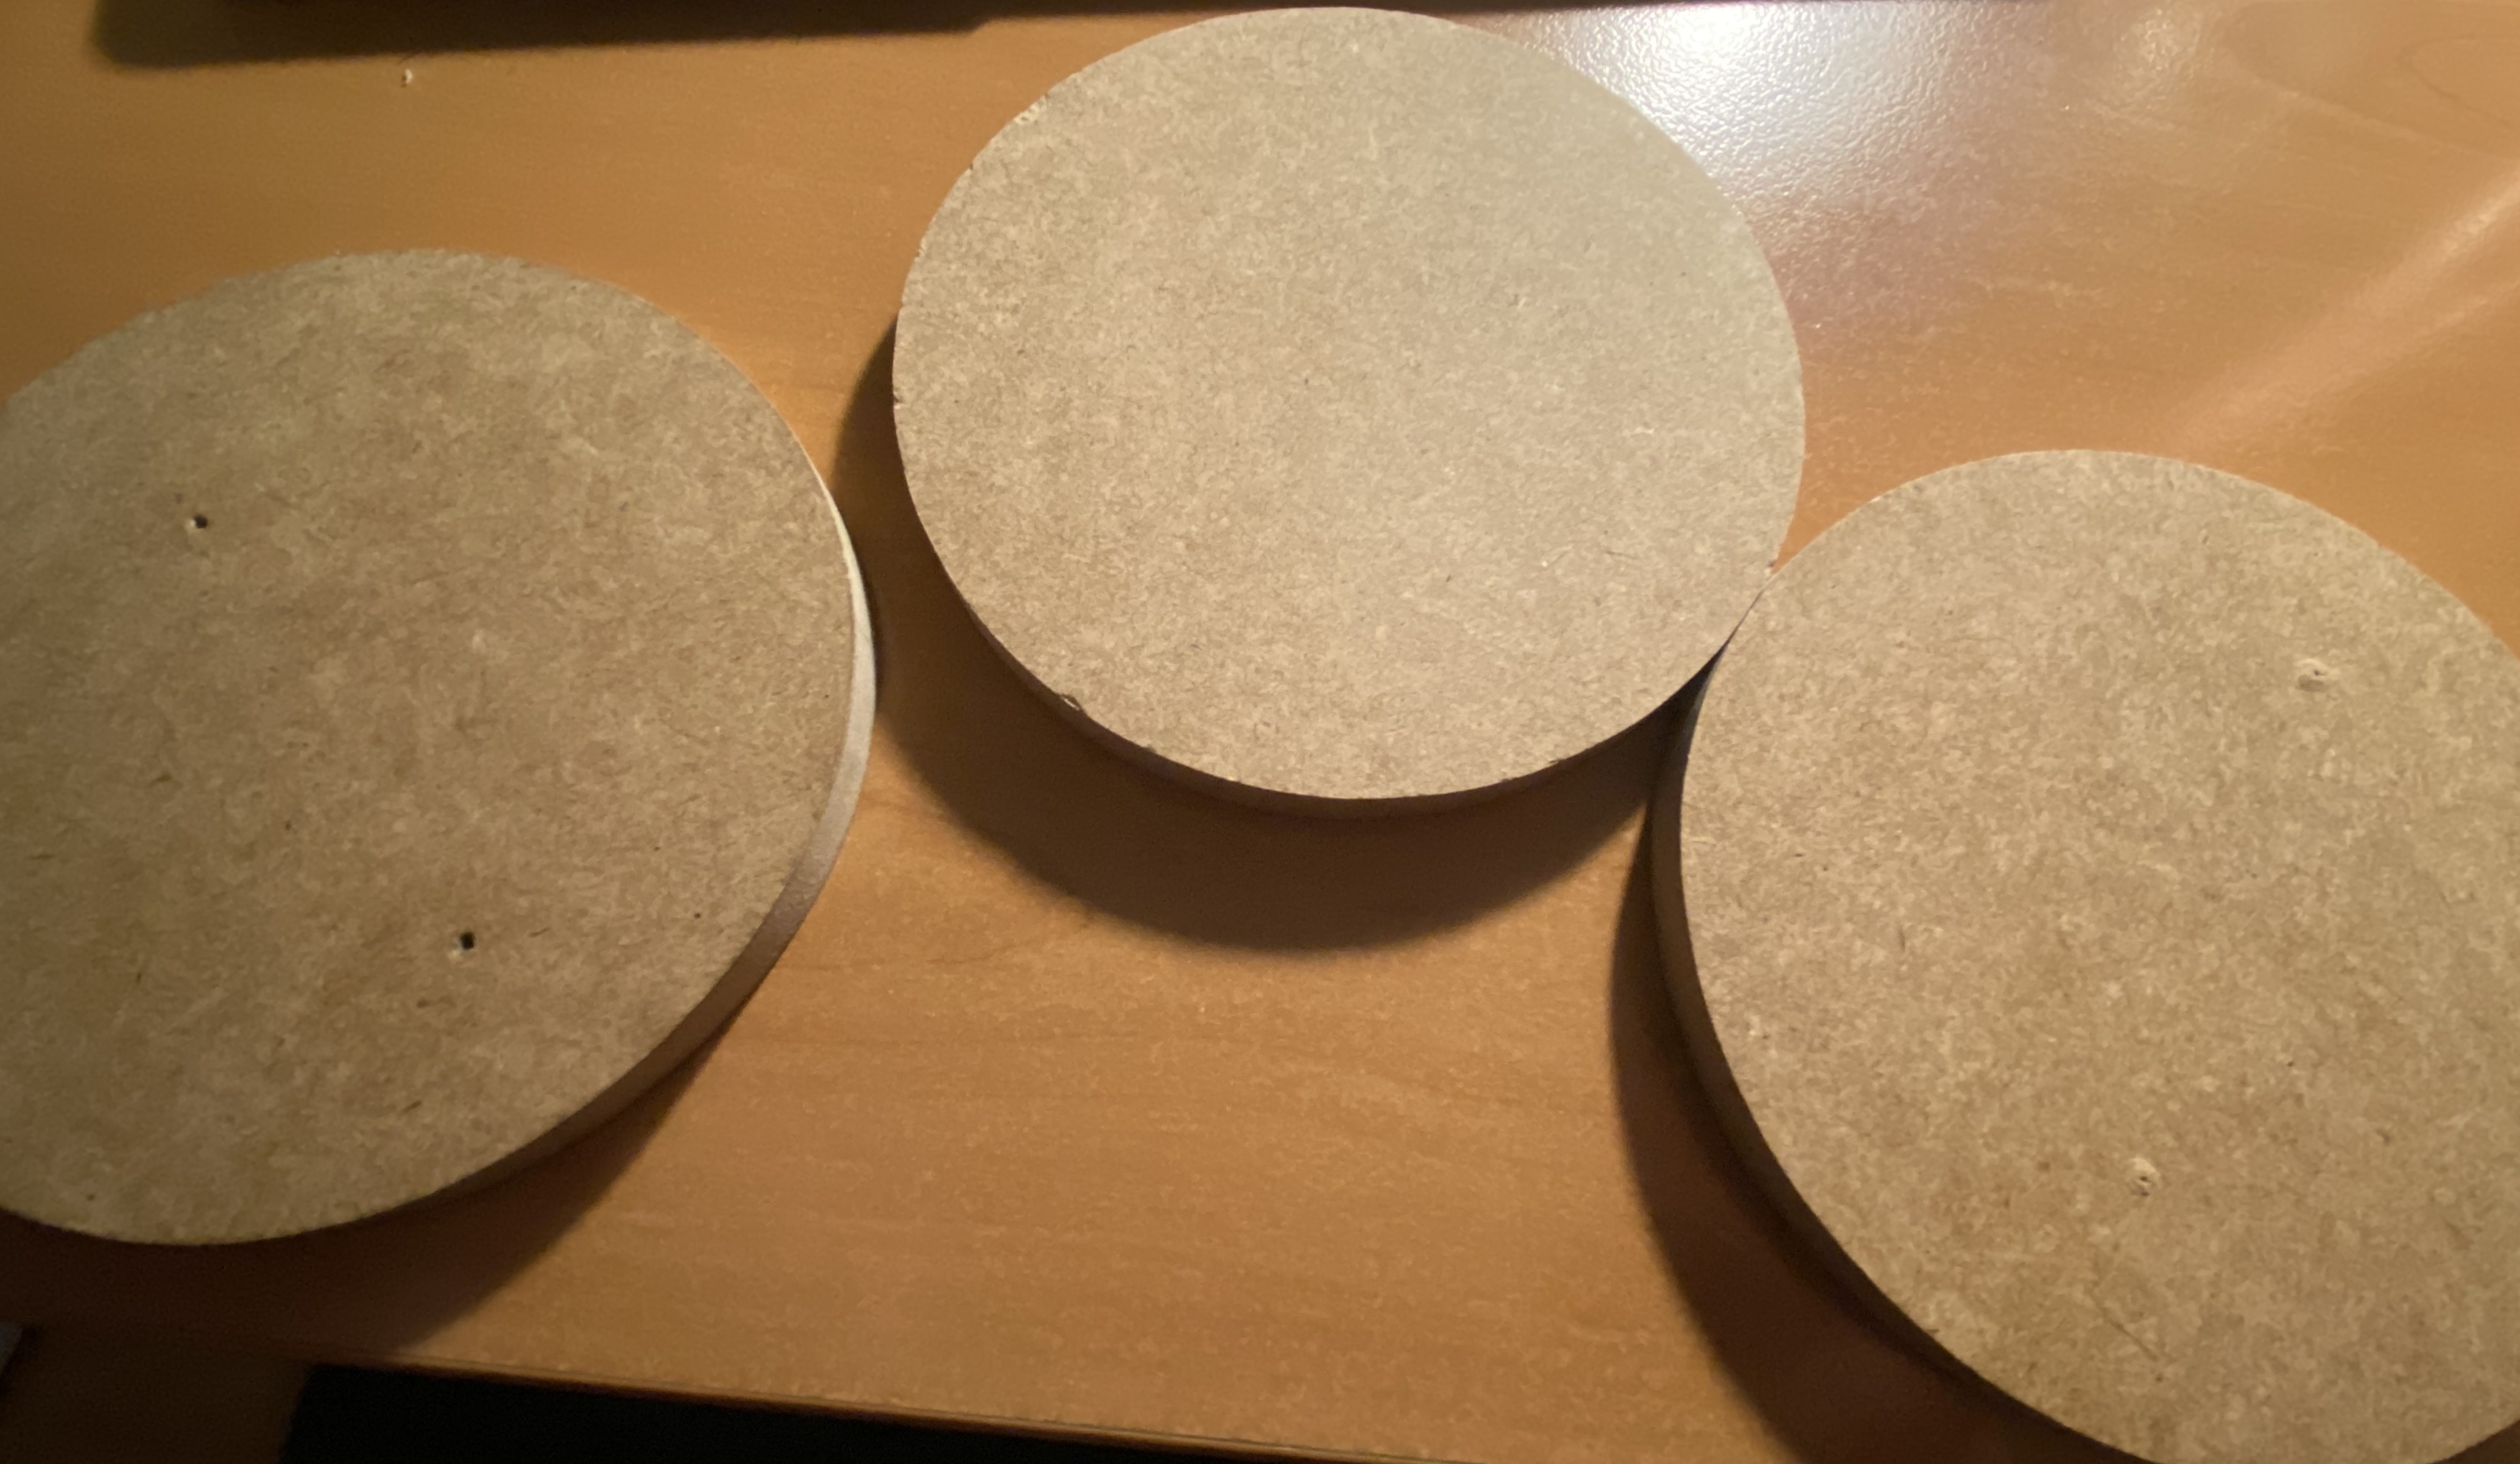
\includegraphics[width=\textwidth]{pads_recortados}
                \caption{Imagen de los pads una vez recortados\label{fig:PadsRecortados}}
            \end{figure}

            Tras ser recortados, el siguiente paso es añadir agujeros en el pad para que pasen los cables del sensor.
            Estos agujeros hacen que, cuando se golpea el pad con la baqueta, se reduzca la posibilidad de dañar los
            cables debido a los golpes. El resultado es el de la figura \ref{fig:PadsAgujeros}

            \newpage

            \begin{figure}[ht]
                \centering
                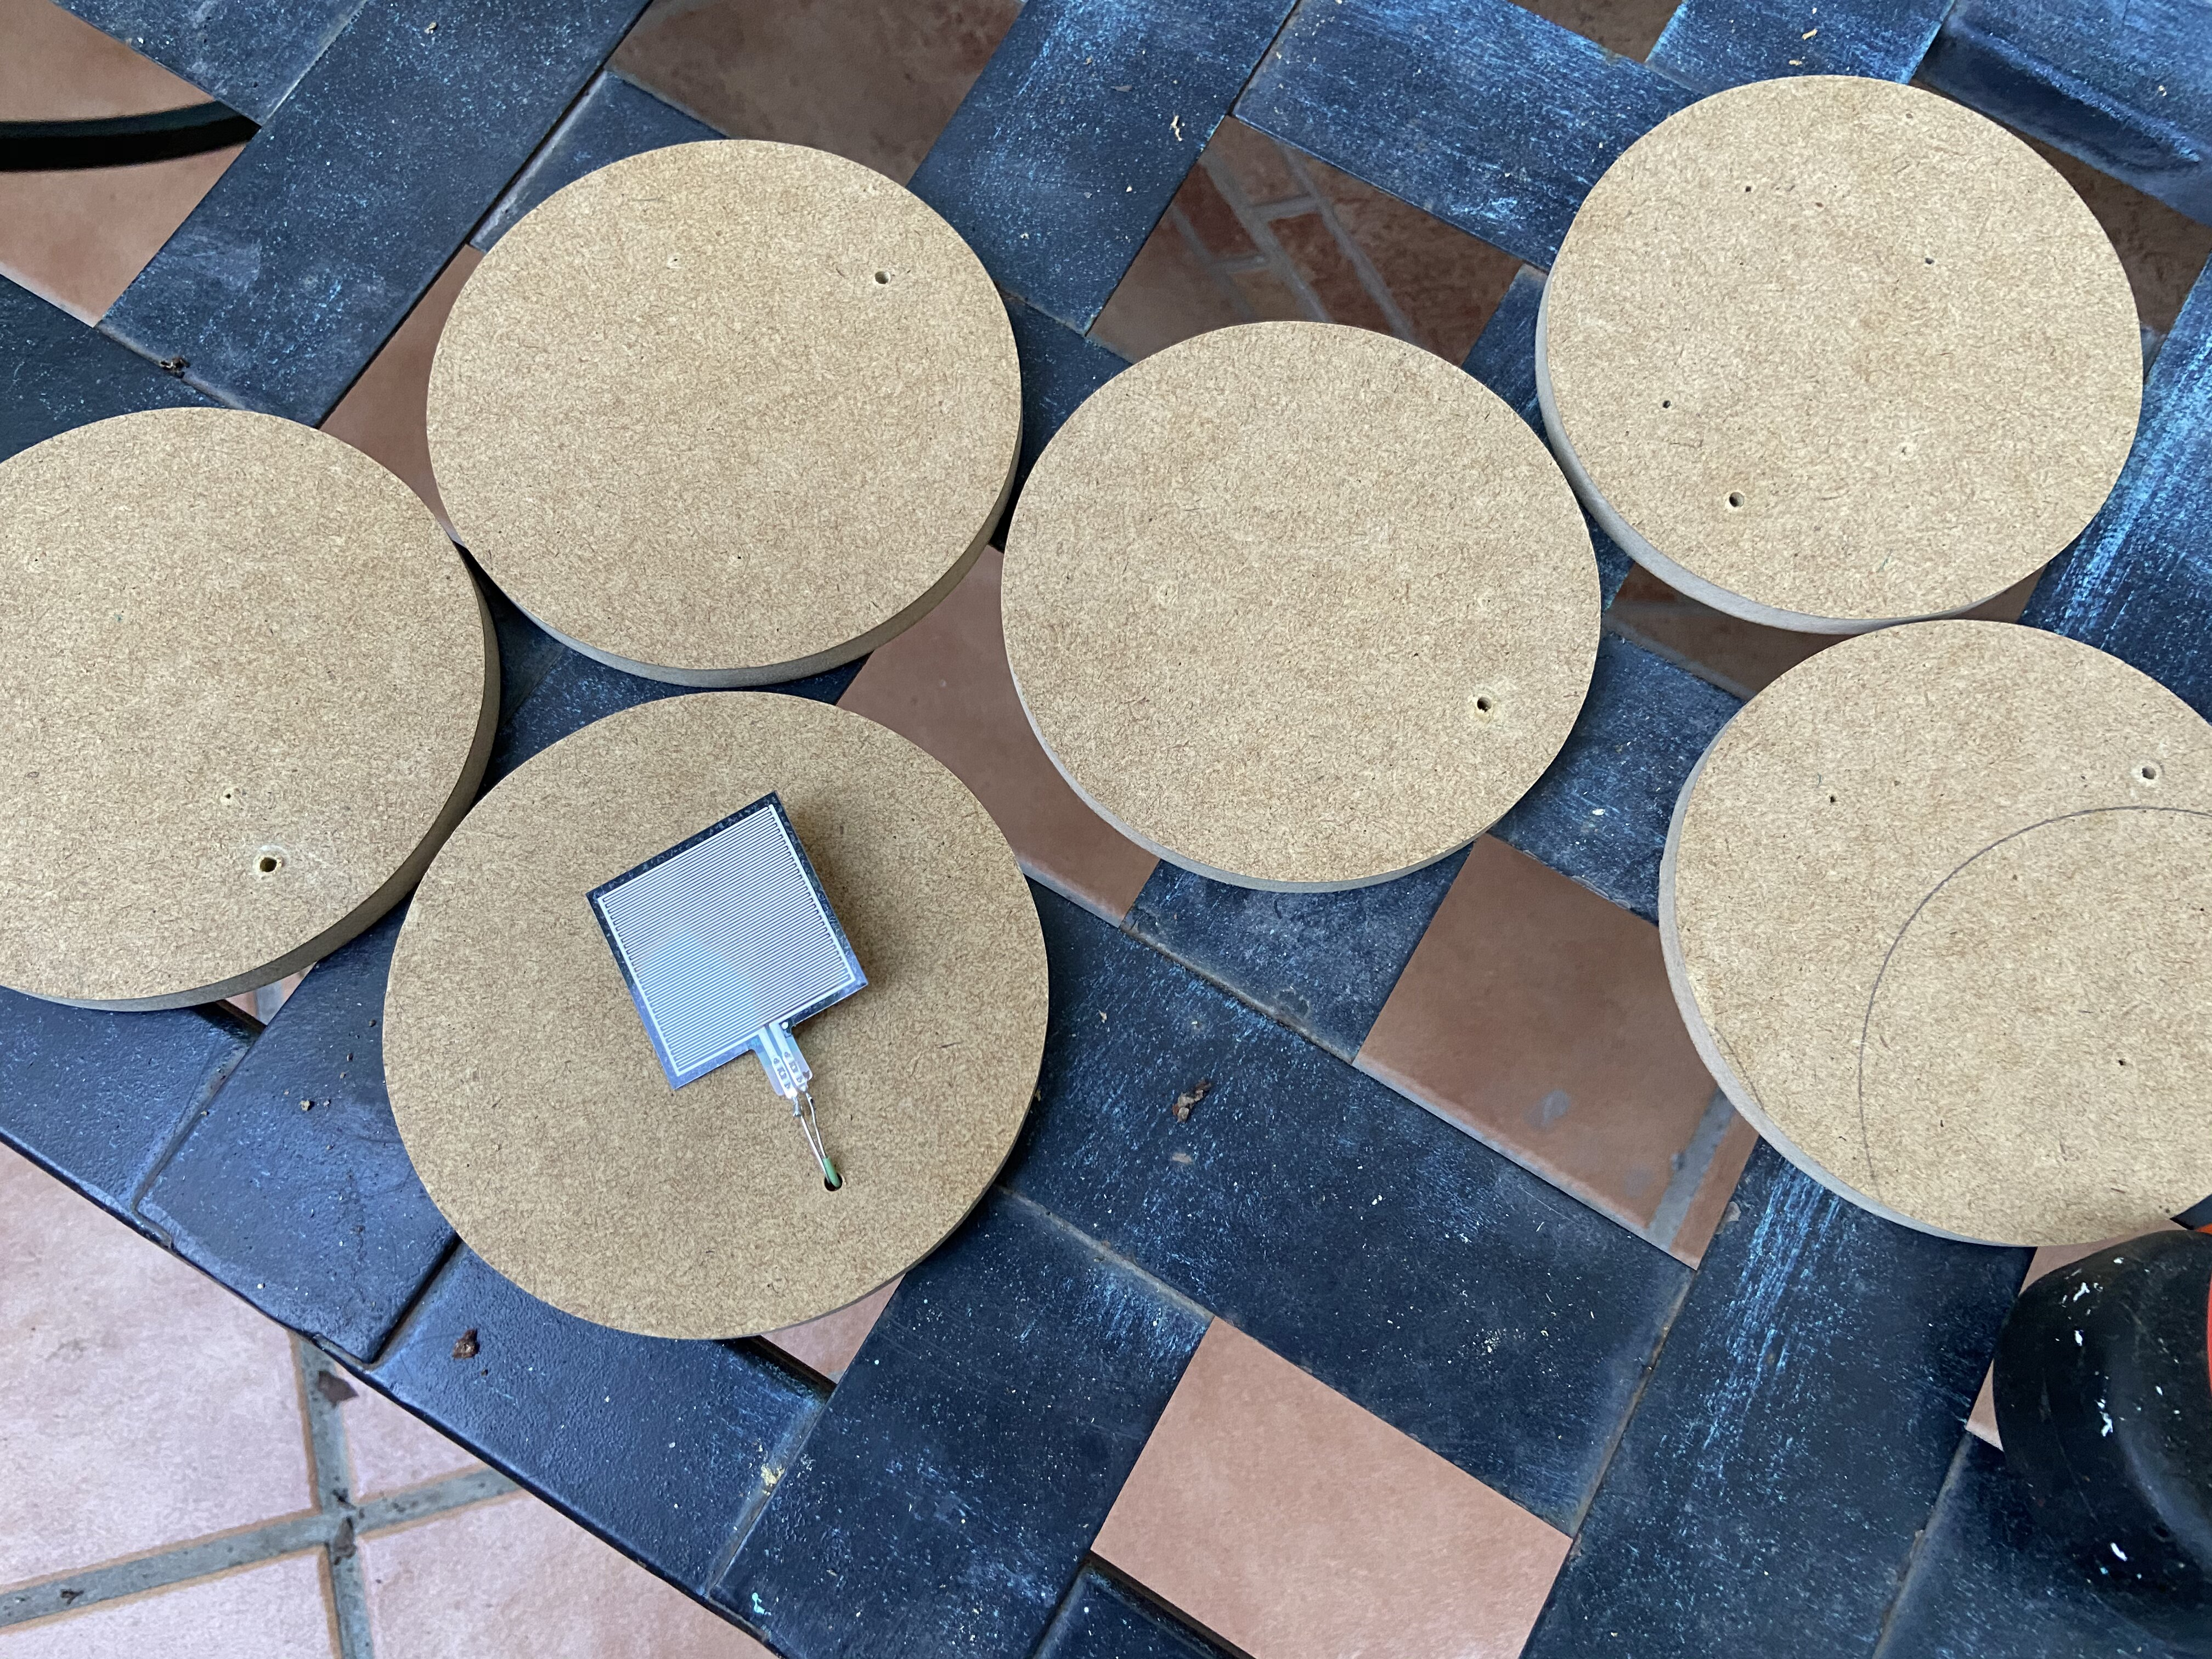
\includegraphics[width=\textwidth]{pads_con_agujeros}
                \caption{Imagen de los pads y un sensor tras añadir los agujeros\label{fig:PadsAgujeros}}
            \end{figure}

            Una vez hecho eso, se añade la gomaeva para proteger los sensores y dar una mayor sensación de realismo al
            ser golpeado con la baqueta.

            --- Imagen aquí ---
            %%%%%%%%%%%%%%%%%%%%%%%%%%%%%%%%%%
            % Imagen de los pad con la gomaeva
            %%%%%%%%%%%%%%%%%%%%%%%%%%%%%%%%%%

        % subsection Construcción (end)

    % section Pads (end)

    \section{Tiempo} % (fold)
    \label{sec:Tiempo}

        Para medir el tiempo que ha llevado realizar este trabajo, se ha utilizado la aplicación
        Clockify \cite{clockify}.\newline

        %%%%%%%%%%%%%%%%%%%%%%%%%%%%%%%%%%%%%%%%%%%%%%%%%%%%%%%%%%%%%%%%%%%%%%%%%%%%%%%%%%%%%%%%%%%%%%%%%%%%%%%%%%%%%%%%
        %%%%%%%%%%%%%%%%%%%%%%%%%%%%%%%%%%%%%%%%%%%%%%%%%%%%%%%%%%%%%%%%%%%%%%%%%%%%%%%%%%%%%%%%%%%%%%%%%%%%%%%%%%%%%%%%
        %%%%%%%%%%%%%%%%%%%%%%%%%%%%%%%%%%%%%%%%%%%%%%%%%%%%%%%%%%%%%%%%%%%%%%%%%%%%%%%%%%%%%%%%%%%%%%%%%%%%%%%%%%%%%%%%
        %%%%%%%%%%%%%%%%%%%%%%%%%%%%%%%%%%%%%%%%%%%%%%%%%%%%%%%%%%%%%%%%%%%%%%%%%%%%%%%%%%%%%%%%%%%%%%%%%%%%%%%%%%%%%%%%
        En total se han utilizado 154 horas y 30 minutos. De estas horas, la división del tiempo ha sido la siguiente:

        \begin{itemize}
            \item Código: 99 horas y 45 minutos
            \item Memoria: 45 horas y 45 minutos
            \item Construcción: 7 horas y 34 minutos
            \item Reuniones con el tutor: 1 hora y 25 minutos
        \end{itemize}
        %%%%%%%%%%%%%%%%%%%%%%%%%%%%%%%%%%%%%%%%%%%%%%%%%%%%%%%%%%%%%%%%%%%%%%%%%%%%%%%%%%%%%%%%%%%%%%%%%%%%%%%%%%%%%%%%
        %%%%%%%%%%%%%%%%%%%%%%%%%%%%%%%%%%%%%%%%%%%%%%%%%%%%%%%%%%%%%%%%%%%%%%%%%%%%%%%%%%%%%%%%%%%%%%%%%%%%%%%%%%%%%%%%
        %%%%%%%%%%%%%%%%%%%%%%%%%%%%%%%%%%%%%%%%%%%%%%%%%%%%%%%%%%%%%%%%%%%%%%%%%%%%%%%%%%%%%%%%%%%%%%%%%%%%%%%%%%%%%%%%
        %%%%%%%%%%%%%%%%%%%%%%%%%%%%%%%%%%%%%%%%%%%%%%%%%%%%%%%%%%%%%%%%%%%%%%%%%%%%%%%%%%%%%%%%%%%%%%%%%%%%%%%%%%%%%%%%

    % section Tiempo (end)

    \section{Coste y presupuesto} % (fold)
    \label{sec:CosteYPresupuesto}

        \subsection{Mano de obra} % (fold)
        \label{sub:ManoDeObra}

            Teniendo en cuenta las horas trabajadas que se han comentado en la sección anterior (\ref{sec:Tiempo}), y el
            sueldo de un ingeniero técnico en Granada, se hará una estimación de cuánto costaría la mano de obra de este
            proyecto.

            Un ingeniero técnico recién salido de la universidad cobra alrededor de 6,81\euro{}/hora. Teniendo esto en
            cuenta, se puede determinar que el coste de la mano de obra sería de unos 1051,80\euro{}.

        % subsection Mano de obra (end)

        \subsection{Materiales} % (fold)
        \label{sub:Materiales}

            \begin{itemize}
                \item Dos hojas de goma eva: 1,20\euro{}
                \item Tres tablas madera MDF 600x300x10 mm: 7,47\euro{}
                \item Cables protoboard: 2,60\euro{}
                \item Sensor de fuerza Exing c18.3: 5,91\euro{}
                \item Cinco sensores de fuerza Exing RP de S40: 50,95\euro{}
                \item Raspberry Pi 3B: 39,95\euro{}
                \item Tarjeta micro SD 8 GB: 5\euro{}
                \item Caja Aukru + cable alimentación: 11,99\euro{}
                \item Arduino Nano: 15,43\euro{} (incluye gastos de envío)
            \end{itemize}

            El coste de los materiales se queda, finalmente, en 140,50\euro{}.

        % subsection Materiales (end)

    % section Coste y presupuesto (end)

% chapter Implementación (end)


%%%%%%%%%%%%%%%%%%%%%%%%%%%%%%%%%%%%%%%%%%%%%%%%%%%%%%%%%%%%%%%%%%%%%%%%%%%%%%%%%
% Resultados y discusión
%%%%%%%%%%%%%%%%%%%%%%%%%%%%%%%%%%%%%%%%%%%%%%%%%%%%%%%%%%%%%%%%%%%%%%%%%%%%%%%%%

\chapter{Resultados y discusión}
\label{cha:ResultadosyDiscusion}

    -> Identifica los aspectos éticos y sociales relacionados con la profesión

    ---- Posiblemente vaya fuera esta sección, no sé muy bien qué añadir ----

% chapter Resultados y discusión (end)

\newpage


%%%%%%%%%%%%%%%%%%%%%%%%%%%%%%%%%%%%%%%%%%%%%%%%%%%%%%%%%%%%%%%%%%%%%%%%%%%%%%%%%
% Conclusiones
%%%%%%%%%%%%%%%%%%%%%%%%%%%%%%%%%%%%%%%%%%%%%%%%%%%%%%%%%%%%%%%%%%%%%%%%%%%%%%%%%

\chapter{Conclusiones}
\label{cha:Conclusiones}

    Llegamos al final del proyecto. Durante los meses que se han invertido en la realización del trabajo, se han
    aprendido varias tecnologías y áreas.

    Se ha aprendido a conectar y programar sensores a placas Raspberry Pi y Arduino. Siguiendo con este tema, se ha
    visto cómo conectar los dos sistemas, para que la Arduino envíe información a la Raspberry Pi para el tratamiento de
    los datos recogidos por los sensores instalados en la Arduino.

    Por otro lado, se ha aprendido a reproducir archivos de sonido en entornos Linux/Unix de manera eficiente y
    simultanea utilizando el lenguaje de programación C.

    Finalmente, se ha alcanzado un resultado que cumple con los objetivos que se marcaron al comienzo del trabajo.
    Utilizando lo aprendido anteriormente, se logra una experiencia de tocar la batería parecida a la realidad,
    incluyendo la construcción de una batería física que poder tocar.

    \section{Trabajo futuro} % (fold)
    \label{sec:TrabajoFuturo}

        ------------ Quitar apartados si se terminan desarrollando ------------

        Durante la realización de este proyecto, ha surgido una serie de ideas que mejorarían la experiencia de tocar la
        batería, pero que, por falta de tiempo, no ha sido posible desarrollar. Las más destables son:

        \begin{itemize}
            \item \textbf{Creación de una interfaz web:} Esta interfaz web podría utilizarse para arrancar y pausar la
            batería de forma sencilla, sin necesidad de entrar a la terminal para ello.
            \item \textbf{Sonidos personalizados:} Añadir un apartado a la interfaz web que permitiera al usuario
            añadir sus propios sonidos personalizados para configurar la batería a su gusto.
            \item \textbf{Aprender canciones:} Mediante una serie de LEDs, que se encienden en el momento preciso, se
            añadiría una canción a la batería y el usuario aprendería a tocarla de forma sencilla. Encendiendo el LED
            del pad que haya que tocar y apagándolo cuando haya sido tocado.
            \item \textbf{Guardar canción tocada:} Grabar lo que toque el usuario durante una cantidad limitada de
            tiempo en un archivo de audio para poder reproducirlo más tarde.
        \end{itemize}

    % section Trabajo futuro (end)

% chapter Conclusiones (end)

\newpage


\addcontentsline{toc}{chapter}{Bibliografía}
\bibliographystyle{plain}
\bibliography{referencias}

\newpage

\end{document}
